\documentclass[twoside]{book}

% Packages required by doxygen
\usepackage{calc}
\usepackage{doxygen}
\usepackage{graphicx}
\usepackage[utf8]{inputenc}
\usepackage{makeidx}
\usepackage{multicol}
\usepackage{multirow}
\usepackage{fixltx2e}
\PassOptionsToPackage{warn}{textcomp}
\usepackage{textcomp}
\usepackage[nointegrals]{wasysym}
\usepackage[table]{xcolor}

% Font selection
\usepackage[T1]{fontenc}
\usepackage{mathptmx}
\usepackage[scaled=.90]{helvet}
\usepackage{courier}
\usepackage{amssymb}
\usepackage{sectsty}
\renewcommand{\familydefault}{\sfdefault}
\allsectionsfont{%
  \fontseries{bc}\selectfont%
  \color{darkgray}%
}
\renewcommand{\DoxyLabelFont}{%
  \fontseries{bc}\selectfont%
  \color{darkgray}%
}
\newcommand{\+}{\discretionary{\mbox{\scriptsize$\hookleftarrow$}}{}{}}

% Page & text layout
\usepackage{geometry}
\geometry{%
  a4paper,%
  top=2.5cm,%
  bottom=2.5cm,%
  left=2.5cm,%
  right=2.5cm%
}
\tolerance=750
\hfuzz=15pt
\hbadness=750
\setlength{\emergencystretch}{15pt}
\setlength{\parindent}{0cm}
\setlength{\parskip}{0.2cm}
\makeatletter
\renewcommand{\paragraph}{%
  \@startsection{paragraph}{4}{0ex}{-1.0ex}{1.0ex}{%
    \normalfont\normalsize\bfseries\SS@parafont%
  }%
}
\renewcommand{\subparagraph}{%
  \@startsection{subparagraph}{5}{0ex}{-1.0ex}{1.0ex}{%
    \normalfont\normalsize\bfseries\SS@subparafont%
  }%
}
\makeatother

% Headers & footers
\usepackage{fancyhdr}
\pagestyle{fancyplain}
\fancyhead[LE]{\fancyplain{}{\bfseries\thepage}}
\fancyhead[CE]{\fancyplain{}{}}
\fancyhead[RE]{\fancyplain{}{\bfseries\leftmark}}
\fancyhead[LO]{\fancyplain{}{\bfseries\rightmark}}
\fancyhead[CO]{\fancyplain{}{}}
\fancyhead[RO]{\fancyplain{}{\bfseries\thepage}}
\fancyfoot[LE]{\fancyplain{}{}}
\fancyfoot[CE]{\fancyplain{}{}}
\fancyfoot[RE]{\fancyplain{}{\bfseries\scriptsize Generated on Fri Apr 17 2015 22\+:17\+:31 for R\+R\+T Simulator 2015 by Doxygen }}
\fancyfoot[LO]{\fancyplain{}{\bfseries\scriptsize Generated on Fri Apr 17 2015 22\+:17\+:31 for R\+R\+T Simulator 2015 by Doxygen }}
\fancyfoot[CO]{\fancyplain{}{}}
\fancyfoot[RO]{\fancyplain{}{}}
\renewcommand{\footrulewidth}{0.4pt}
\renewcommand{\chaptermark}[1]{%
  \markboth{#1}{}%
}
\renewcommand{\sectionmark}[1]{%
  \markright{\thesection\ #1}%
}

% Indices & bibliography
\usepackage{natbib}
\usepackage[titles]{tocloft}
\setcounter{tocdepth}{3}
\setcounter{secnumdepth}{5}
\makeindex

% Hyperlinks (required, but should be loaded last)
\usepackage{ifpdf}
\ifpdf
  \usepackage[pdftex,pagebackref=true]{hyperref}
\else
  \usepackage[ps2pdf,pagebackref=true]{hyperref}
\fi
\hypersetup{%
  colorlinks=true,%
  linkcolor=blue,%
  citecolor=blue,%
  unicode%
}

% Custom commands
\newcommand{\clearemptydoublepage}{%
  \newpage{\pagestyle{empty}\cleardoublepage}%
}


%===== C O N T E N T S =====

\begin{document}

% Titlepage & ToC
\hypersetup{pageanchor=false,
             bookmarks=true,
             bookmarksnumbered=true,
             pdfencoding=unicode
            }
\pagenumbering{roman}
\begin{titlepage}
\vspace*{7cm}
\begin{center}%
{\Large R\+R\+T Simulator 2015 }\\
\vspace*{1cm}
{\large Generated by Doxygen 1.8.7}\\
\vspace*{0.5cm}
{\small Fri Apr 17 2015 22:17:31}\\
\end{center}
\end{titlepage}
\clearemptydoublepage
\tableofcontents
\clearemptydoublepage
\pagenumbering{arabic}
\hypersetup{pageanchor=true}

%--- Begin generated contents ---
\chapter{Namespace Index}
\section{Namespace List}
Here is a list of all namespaces with brief descriptions\+:\begin{DoxyCompactList}
\item\contentsline{section}{\hyperlink{namespacesf}{sf} }{\pageref{namespacesf}}{}
\end{DoxyCompactList}

\chapter{Class Index}
\section{Class List}
Here are the classes, structs, unions and interfaces with brief descriptions\+:\begin{DoxyCompactList}
\item\contentsline{section}{\hyperlink{classLevelData}{Level\+Data} \\*Represents a loaded level, this contains the dimensions and tiles of a level which can be used for A\+I algorithms. }{\pageref{classLevelData}}{}
\item\contentsline{section}{\hyperlink{classLevelViewer}{Level\+Viewer} \\*A class used to display the contents of a \hyperlink{classLevelData}{Level\+Data} object on screen. }{\pageref{classLevelViewer}}{}
\item\contentsline{section}{\hyperlink{classRRT}{R\+R\+T} \\*A class which creates an \hyperlink{classRRT}{R\+R\+T} tree when given a map and a start and end point. }{\pageref{classRRT}}{}
\item\contentsline{section}{\hyperlink{classRRTDemo}{R\+R\+T\+Demo} \\*A demo application which loads in level data from a file and uses the \hyperlink{classRRT}{R\+R\+T} algorithm to implement path finding. }{\pageref{classRRTDemo}}{}
\item\contentsline{section}{\hyperlink{classTree}{Tree$<$ T $>$} \\*A tree data structure containing a parent and an unlimited number of children. }{\pageref{classTree}}{}
\end{DoxyCompactList}

\chapter{File Index}
\section{File List}
Here is a list of all files with brief descriptions\+:\begin{DoxyCompactList}
\item\contentsline{section}{U\+:/\+Work/\+Year2/\+G\+E\+C/\+A\+I/\+Source/\hyperlink{RRTDemo_8cpp}{R\+R\+T\+Demo.\+cpp} }{\pageref{RRTDemo_8cpp}}{}
\item\contentsline{section}{U\+:/\+Work/\+Year2/\+G\+E\+C/\+A\+I/\+Source/\hyperlink{RRTDemo_8hpp}{R\+R\+T\+Demo.\+hpp} }{\pageref{RRTDemo_8hpp}}{}
\item\contentsline{section}{U\+:/\+Work/\+Year2/\+G\+E\+C/\+A\+I/\+Source/\+Level/\hyperlink{LevelData_8cpp}{Level\+Data.\+cpp} }{\pageref{LevelData_8cpp}}{}
\item\contentsline{section}{U\+:/\+Work/\+Year2/\+G\+E\+C/\+A\+I/\+Source/\+Level/\hyperlink{LevelData_8hpp}{Level\+Data.\+hpp} }{\pageref{LevelData_8hpp}}{}
\item\contentsline{section}{U\+:/\+Work/\+Year2/\+G\+E\+C/\+A\+I/\+Source/\+Level/\hyperlink{LevelViewer_8cpp}{Level\+Viewer.\+cpp} }{\pageref{LevelViewer_8cpp}}{}
\item\contentsline{section}{U\+:/\+Work/\+Year2/\+G\+E\+C/\+A\+I/\+Source/\+Level/\hyperlink{LevelViewer_8hpp}{Level\+Viewer.\+hpp} }{\pageref{LevelViewer_8hpp}}{}
\item\contentsline{section}{U\+:/\+Work/\+Year2/\+G\+E\+C/\+A\+I/\+Source/\+R\+R\+T/\hyperlink{RRT_8cpp}{R\+R\+T.\+cpp} }{\pageref{RRT_8cpp}}{}
\item\contentsline{section}{U\+:/\+Work/\+Year2/\+G\+E\+C/\+A\+I/\+Source/\+R\+R\+T/\hyperlink{RRT_8hpp}{R\+R\+T.\+hpp} }{\pageref{RRT_8hpp}}{}
\item\contentsline{section}{U\+:/\+Work/\+Year2/\+G\+E\+C/\+A\+I/\+Source/\+R\+R\+T/\hyperlink{Tree_8hpp}{Tree.\+hpp} }{\pageref{Tree_8hpp}}{}
\end{DoxyCompactList}

\chapter{Namespace Documentation}
\hypertarget{namespacesf}{\section{sf Namespace Reference}
\label{namespacesf}\index{sf@{sf}}
}

\chapter{Class Documentation}
\hypertarget{classLevelData}{\section{Level\+Data Class Reference}
\label{classLevelData}\index{Level\+Data@{Level\+Data}}
}


Represents a loaded level, this contains the dimensions and tiles of a level which can be used for A\+I algorithms.  




{\ttfamily \#include $<$Level\+Data.\+hpp$>$}

\subsection*{Public Member Functions}
\begin{DoxyCompactItemize}
\item 
\hyperlink{classLevelData_a278138fae5c623551b7b90c28e75f056}{Level\+Data} (const std\+::string \&file)
\begin{DoxyCompactList}\small\item\em Constructs a \hyperlink{classLevelData}{Level\+Data} object from the given file containing level information. Exceptions can be thrown. \end{DoxyCompactList}\item 
\hyperlink{classLevelData_af56cf70c4f4991db88ac77c5c2e5b2c5}{Level\+Data} (\hyperlink{classLevelData}{Level\+Data} \&\&move)
\item 
\hyperlink{classLevelData}{Level\+Data} \& \hyperlink{classLevelData_aa979caad1a51d2dd77d5cf6b88c83484}{operator=} (\hyperlink{classLevelData}{Level\+Data} \&\&move)
\item 
\hyperlink{classLevelData_a3ca3249521b88b01f2aab308ce1c3097}{Level\+Data} (const \hyperlink{classLevelData}{Level\+Data} \&copy)=default
\item 
\hyperlink{classLevelData}{Level\+Data} \& \hyperlink{classLevelData_a1ac815425733ec660357d3b594ecdffa}{operator=} (const \hyperlink{classLevelData}{Level\+Data} \&copy)=default
\item 
\hyperlink{classLevelData_a534a1a46628043bd85fcc4838ebe45cf}{$\sim$\+Level\+Data} ()=default
\item 
unsigned int \hyperlink{classLevelData_ad169e7a33905caaf20ad6057166f40c3}{get\+Width} () const 
\begin{DoxyCompactList}\small\item\em Gets the tile width of the level. \end{DoxyCompactList}\item 
unsigned int \hyperlink{classLevelData_aa58248c6dac7cef0b240df372ac09f34}{get\+Height} () const 
\begin{DoxyCompactList}\small\item\em Gets the tile height of the level. \end{DoxyCompactList}\item 
unsigned int \hyperlink{classLevelData_a25eb0194cebc5d67508e3c8dbefadc11}{get\+Tile\+Count} () const 
\begin{DoxyCompactList}\small\item\em Gets the total number of loaded tiles in the level. \end{DoxyCompactList}\item 
const std\+::string \& \hyperlink{classLevelData_a6c1c2be838a5b7e55ce6ff0e804ab09d}{get\+File\+Location} () const 
\begin{DoxyCompactList}\small\item\em Gets the file location of the loaded level data. \end{DoxyCompactList}\item 
\hyperlink{LevelData_8hpp_a47dee72188473c57343127b1a5843398}{Tile\+Type} \hyperlink{classLevelData_a290837e4d45e346b69bc805362a31e69}{get\+Tile} (const unsigned int index) const 
\begin{DoxyCompactList}\small\item\em Obtains the type for the given tile. \end{DoxyCompactList}\item 
\hyperlink{LevelData_8hpp_a47dee72188473c57343127b1a5843398}{Tile\+Type} \hyperlink{classLevelData_a899fadb559d257e0457bbe5778498f03}{get\+Tile} (const unsigned int x, const unsigned int y) const 
\begin{DoxyCompactList}\small\item\em Obtains the type for the tile at the given co-\/ordinate. \end{DoxyCompactList}\item 
void \hyperlink{classLevelData_a1ec79101880076ae4291fcdda279633b}{load\+From\+File} (const std\+::string \&file)
\begin{DoxyCompactList}\small\item\em Load level data from a file at the given location. If an error occurs an exception will be thrown. \end{DoxyCompactList}\end{DoxyCompactItemize}
\subsection*{Private Member Functions}
\begin{DoxyCompactItemize}
\item 
void \hyperlink{classLevelData_a68e8ac8397ac430ebd28f3db2cd2020a}{read\+Header} (std\+::ifstream \&stream)
\begin{DoxyCompactList}\small\item\em Reads the header of a map file and prepares the tile data accordingly. Throws exceptions if the header is invalid. \end{DoxyCompactList}\item 
void \hyperlink{classLevelData_ad9e4687d526e6b503617338279aabb33}{read\+Level} (std\+::ifstream \&stream)
\begin{DoxyCompactList}\small\item\em Reads the tile data of a level from a given stream. Throws exceptions upon errors. \end{DoxyCompactList}\item 
\hyperlink{LevelData_8hpp_a47dee72188473c57343127b1a5843398}{Tile\+Type} \hyperlink{classLevelData_a22aa59bed8da92af1921066eeef30a19}{determine\+Tile\+Type} (const char tile) const 
\begin{DoxyCompactList}\small\item\em Determines the Tile\+Type which corresponds to the given character. \end{DoxyCompactList}\end{DoxyCompactItemize}
\subsection*{Private Attributes}
\begin{DoxyCompactItemize}
\item 
unsigned int \hyperlink{classLevelData_af2aaac4914ff63edf43f93592e117abf}{m\+\_\+width} \{ 0 \}
\begin{DoxyCompactList}\small\item\em The number of tiles that make up the level width. \end{DoxyCompactList}\item 
unsigned int \hyperlink{classLevelData_af6895162dbf2aae99d81f2bd39bfd0fc}{m\+\_\+height} \{ 0 \}
\begin{DoxyCompactList}\small\item\em The number of tiles that make up the level height. \end{DoxyCompactList}\item 
std\+::string \hyperlink{classLevelData_a65e6372aea8e8d29fe9a554653a1ad24}{m\+\_\+map\+File} = \char`\"{}\char`\"{}
\begin{DoxyCompactList}\small\item\em The file location where the level data was loaded from. \end{DoxyCompactList}\item 
std\+::vector$<$ \hyperlink{LevelData_8hpp_a47dee72188473c57343127b1a5843398}{Tile\+Type} $>$ \hyperlink{classLevelData_a32b98877ba76059d320053f55dd97051}{m\+\_\+tile\+Data} \{ \}
\begin{DoxyCompactList}\small\item\em The type of every tile on the level. \end{DoxyCompactList}\end{DoxyCompactItemize}


\subsection{Detailed Description}
Represents a loaded level, this contains the dimensions and tiles of a level which can be used for A\+I algorithms. 



Definition at line 27 of file Level\+Data.\+hpp.



\subsection{Constructor \& Destructor Documentation}
\hypertarget{classLevelData_a278138fae5c623551b7b90c28e75f056}{\index{Level\+Data@{Level\+Data}!Level\+Data@{Level\+Data}}
\index{Level\+Data@{Level\+Data}!Level\+Data@{Level\+Data}}
\subsubsection[{Level\+Data}]{\setlength{\rightskip}{0pt plus 5cm}Level\+Data\+::\+Level\+Data (
\begin{DoxyParamCaption}
\item[{const std\+::string \&}]{file}
\end{DoxyParamCaption}
)}}\label{classLevelData_a278138fae5c623551b7b90c28e75f056}


Constructs a \hyperlink{classLevelData}{Level\+Data} object from the given file containing level information. Exceptions can be thrown. 


\begin{DoxyParams}{Parameters}
{\em file} & The file to load from. \\
\hline
\end{DoxyParams}


Definition at line 16 of file Level\+Data.\+cpp.

\hypertarget{classLevelData_af56cf70c4f4991db88ac77c5c2e5b2c5}{\index{Level\+Data@{Level\+Data}!Level\+Data@{Level\+Data}}
\index{Level\+Data@{Level\+Data}!Level\+Data@{Level\+Data}}
\subsubsection[{Level\+Data}]{\setlength{\rightskip}{0pt plus 5cm}Level\+Data\+::\+Level\+Data (
\begin{DoxyParamCaption}
\item[{{\bf Level\+Data} \&\&}]{move}
\end{DoxyParamCaption}
)}}\label{classLevelData_af56cf70c4f4991db88ac77c5c2e5b2c5}


Definition at line 22 of file Level\+Data.\+cpp.

\hypertarget{classLevelData_a3ca3249521b88b01f2aab308ce1c3097}{\index{Level\+Data@{Level\+Data}!Level\+Data@{Level\+Data}}
\index{Level\+Data@{Level\+Data}!Level\+Data@{Level\+Data}}
\subsubsection[{Level\+Data}]{\setlength{\rightskip}{0pt plus 5cm}Level\+Data\+::\+Level\+Data (
\begin{DoxyParamCaption}
\item[{const {\bf Level\+Data} \&}]{copy}
\end{DoxyParamCaption}
)\hspace{0.3cm}{\ttfamily [default]}}}\label{classLevelData_a3ca3249521b88b01f2aab308ce1c3097}
\hypertarget{classLevelData_a534a1a46628043bd85fcc4838ebe45cf}{\index{Level\+Data@{Level\+Data}!````~Level\+Data@{$\sim$\+Level\+Data}}
\index{````~Level\+Data@{$\sim$\+Level\+Data}!Level\+Data@{Level\+Data}}
\subsubsection[{$\sim$\+Level\+Data}]{\setlength{\rightskip}{0pt plus 5cm}Level\+Data\+::$\sim$\+Level\+Data (
\begin{DoxyParamCaption}
{}
\end{DoxyParamCaption}
)\hspace{0.3cm}{\ttfamily [default]}}}\label{classLevelData_a534a1a46628043bd85fcc4838ebe45cf}


\subsection{Member Function Documentation}
\hypertarget{classLevelData_aa979caad1a51d2dd77d5cf6b88c83484}{\index{Level\+Data@{Level\+Data}!operator=@{operator=}}
\index{operator=@{operator=}!Level\+Data@{Level\+Data}}
\subsubsection[{operator=}]{\setlength{\rightskip}{0pt plus 5cm}{\bf Level\+Data} \& Level\+Data\+::operator= (
\begin{DoxyParamCaption}
\item[{{\bf Level\+Data} \&\&}]{move}
\end{DoxyParamCaption}
)}}\label{classLevelData_aa979caad1a51d2dd77d5cf6b88c83484}


Definition at line 28 of file Level\+Data.\+cpp.

\hypertarget{classLevelData_a1ac815425733ec660357d3b594ecdffa}{\index{Level\+Data@{Level\+Data}!operator=@{operator=}}
\index{operator=@{operator=}!Level\+Data@{Level\+Data}}
\subsubsection[{operator=}]{\setlength{\rightskip}{0pt plus 5cm}{\bf Level\+Data}\& Level\+Data\+::operator= (
\begin{DoxyParamCaption}
\item[{const {\bf Level\+Data} \&}]{copy}
\end{DoxyParamCaption}
)\hspace{0.3cm}{\ttfamily [default]}}}\label{classLevelData_a1ac815425733ec660357d3b594ecdffa}
\hypertarget{classLevelData_ad169e7a33905caaf20ad6057166f40c3}{\index{Level\+Data@{Level\+Data}!get\+Width@{get\+Width}}
\index{get\+Width@{get\+Width}!Level\+Data@{Level\+Data}}
\subsubsection[{get\+Width}]{\setlength{\rightskip}{0pt plus 5cm}unsigned int Level\+Data\+::get\+Width (
\begin{DoxyParamCaption}
{}
\end{DoxyParamCaption}
) const\hspace{0.3cm}{\ttfamily [inline]}}}\label{classLevelData_ad169e7a33905caaf20ad6057166f40c3}


Gets the tile width of the level. 



Definition at line 52 of file Level\+Data.\+hpp.



Here is the caller graph for this function\+:
\nopagebreak
\begin{figure}[H]
\begin{center}
\leavevmode
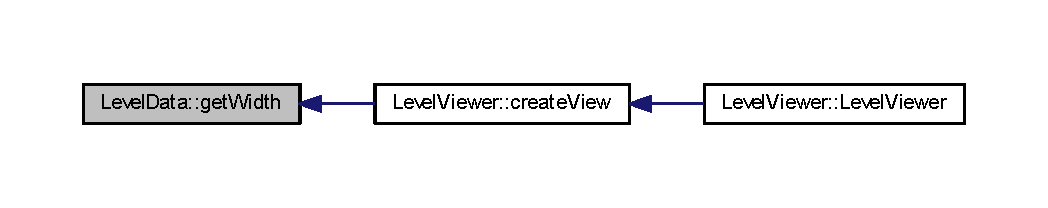
\includegraphics[width=350pt]{classLevelData_ad169e7a33905caaf20ad6057166f40c3_icgraph}
\end{center}
\end{figure}


\hypertarget{classLevelData_aa58248c6dac7cef0b240df372ac09f34}{\index{Level\+Data@{Level\+Data}!get\+Height@{get\+Height}}
\index{get\+Height@{get\+Height}!Level\+Data@{Level\+Data}}
\subsubsection[{get\+Height}]{\setlength{\rightskip}{0pt plus 5cm}unsigned int Level\+Data\+::get\+Height (
\begin{DoxyParamCaption}
{}
\end{DoxyParamCaption}
) const\hspace{0.3cm}{\ttfamily [inline]}}}\label{classLevelData_aa58248c6dac7cef0b240df372ac09f34}


Gets the tile height of the level. 



Definition at line 55 of file Level\+Data.\+hpp.



Here is the caller graph for this function\+:
\nopagebreak
\begin{figure}[H]
\begin{center}
\leavevmode
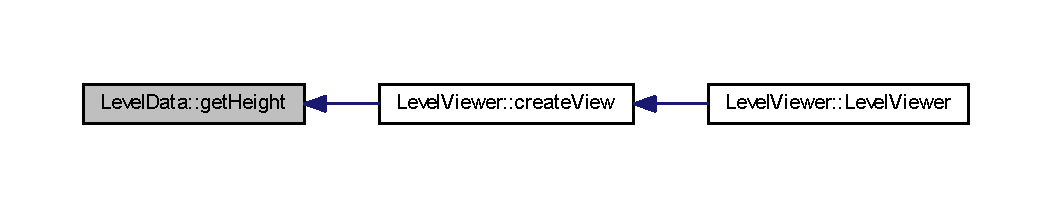
\includegraphics[width=350pt]{classLevelData_aa58248c6dac7cef0b240df372ac09f34_icgraph}
\end{center}
\end{figure}


\hypertarget{classLevelData_a25eb0194cebc5d67508e3c8dbefadc11}{\index{Level\+Data@{Level\+Data}!get\+Tile\+Count@{get\+Tile\+Count}}
\index{get\+Tile\+Count@{get\+Tile\+Count}!Level\+Data@{Level\+Data}}
\subsubsection[{get\+Tile\+Count}]{\setlength{\rightskip}{0pt plus 5cm}unsigned int Level\+Data\+::get\+Tile\+Count (
\begin{DoxyParamCaption}
{}
\end{DoxyParamCaption}
) const\hspace{0.3cm}{\ttfamily [inline]}}}\label{classLevelData_a25eb0194cebc5d67508e3c8dbefadc11}


Gets the total number of loaded tiles in the level. 



Definition at line 58 of file Level\+Data.\+hpp.



Here is the caller graph for this function\+:
\nopagebreak
\begin{figure}[H]
\begin{center}
\leavevmode
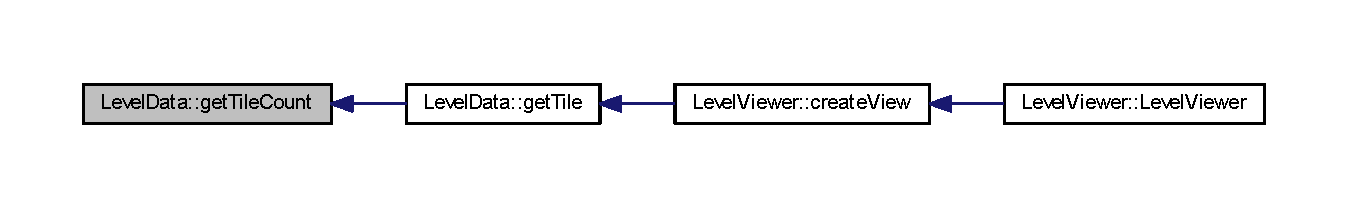
\includegraphics[width=350pt]{classLevelData_a25eb0194cebc5d67508e3c8dbefadc11_icgraph}
\end{center}
\end{figure}


\hypertarget{classLevelData_a6c1c2be838a5b7e55ce6ff0e804ab09d}{\index{Level\+Data@{Level\+Data}!get\+File\+Location@{get\+File\+Location}}
\index{get\+File\+Location@{get\+File\+Location}!Level\+Data@{Level\+Data}}
\subsubsection[{get\+File\+Location}]{\setlength{\rightskip}{0pt plus 5cm}const std\+::string\& Level\+Data\+::get\+File\+Location (
\begin{DoxyParamCaption}
{}
\end{DoxyParamCaption}
) const\hspace{0.3cm}{\ttfamily [inline]}}}\label{classLevelData_a6c1c2be838a5b7e55ce6ff0e804ab09d}


Gets the file location of the loaded level data. 



Definition at line 61 of file Level\+Data.\+hpp.

\hypertarget{classLevelData_a290837e4d45e346b69bc805362a31e69}{\index{Level\+Data@{Level\+Data}!get\+Tile@{get\+Tile}}
\index{get\+Tile@{get\+Tile}!Level\+Data@{Level\+Data}}
\subsubsection[{get\+Tile}]{\setlength{\rightskip}{0pt plus 5cm}{\bf Tile\+Type} Level\+Data\+::get\+Tile (
\begin{DoxyParamCaption}
\item[{const unsigned int}]{index}
\end{DoxyParamCaption}
) const}}\label{classLevelData_a290837e4d45e346b69bc805362a31e69}


Obtains the type for the given tile. 


\begin{DoxyParams}{Parameters}
{\em index} & The index of the tile. \\
\hline
\end{DoxyParams}


Definition at line 52 of file Level\+Data.\+cpp.



Here is the caller graph for this function\+:
\nopagebreak
\begin{figure}[H]
\begin{center}
\leavevmode
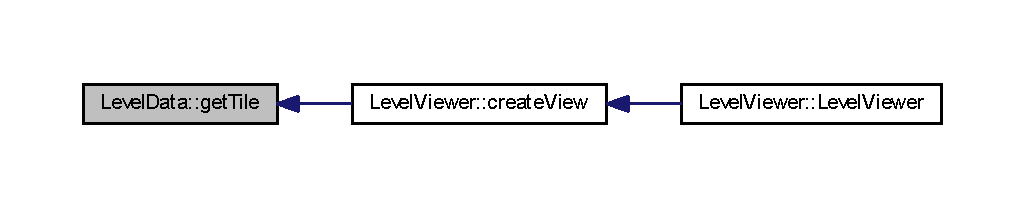
\includegraphics[width=350pt]{classLevelData_a290837e4d45e346b69bc805362a31e69_icgraph}
\end{center}
\end{figure}


\hypertarget{classLevelData_a899fadb559d257e0457bbe5778498f03}{\index{Level\+Data@{Level\+Data}!get\+Tile@{get\+Tile}}
\index{get\+Tile@{get\+Tile}!Level\+Data@{Level\+Data}}
\subsubsection[{get\+Tile}]{\setlength{\rightskip}{0pt plus 5cm}{\bf Tile\+Type} Level\+Data\+::get\+Tile (
\begin{DoxyParamCaption}
\item[{const unsigned int}]{x, }
\item[{const unsigned int}]{y}
\end{DoxyParamCaption}
) const}}\label{classLevelData_a899fadb559d257e0457bbe5778498f03}


Obtains the type for the tile at the given co-\/ordinate. 


\begin{DoxyParams}{Parameters}
{\em x} & The X co-\/ordinate of the tile. \\
\hline
{\em y} & The Y co-\/ordinate of the tile. \\
\hline
\end{DoxyParams}


Definition at line 61 of file Level\+Data.\+cpp.

\hypertarget{classLevelData_a1ec79101880076ae4291fcdda279633b}{\index{Level\+Data@{Level\+Data}!load\+From\+File@{load\+From\+File}}
\index{load\+From\+File@{load\+From\+File}!Level\+Data@{Level\+Data}}
\subsubsection[{load\+From\+File}]{\setlength{\rightskip}{0pt plus 5cm}void Level\+Data\+::load\+From\+File (
\begin{DoxyParamCaption}
\item[{const std\+::string \&}]{file}
\end{DoxyParamCaption}
)}}\label{classLevelData_a1ec79101880076ae4291fcdda279633b}


Load level data from a file at the given location. If an error occurs an exception will be thrown. 


\begin{DoxyParams}{Parameters}
{\em file} & The file location to load from. \\
\hline
\end{DoxyParams}


Definition at line 70 of file Level\+Data.\+cpp.



Here is the caller graph for this function\+:
\nopagebreak
\begin{figure}[H]
\begin{center}
\leavevmode
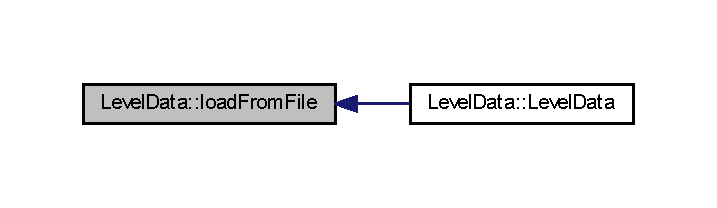
\includegraphics[width=344pt]{classLevelData_a1ec79101880076ae4291fcdda279633b_icgraph}
\end{center}
\end{figure}


\hypertarget{classLevelData_a68e8ac8397ac430ebd28f3db2cd2020a}{\index{Level\+Data@{Level\+Data}!read\+Header@{read\+Header}}
\index{read\+Header@{read\+Header}!Level\+Data@{Level\+Data}}
\subsubsection[{read\+Header}]{\setlength{\rightskip}{0pt plus 5cm}void Level\+Data\+::read\+Header (
\begin{DoxyParamCaption}
\item[{std\+::ifstream \&}]{stream}
\end{DoxyParamCaption}
)\hspace{0.3cm}{\ttfamily [private]}}}\label{classLevelData_a68e8ac8397ac430ebd28f3db2cd2020a}


Reads the header of a map file and prepares the tile data accordingly. Throws exceptions if the header is invalid. 


\begin{DoxyParams}{Parameters}
{\em stream} & An open file stream to read from. \\
\hline
\end{DoxyParams}
The header is in the following format\+: \char`\"{}type blah\char`\"{}, ignore this. \char`\"{}height blah\char`\"{}, gives us the height value. \char`\"{}width blah\char`\"{}, gives us the width value. \char`\"{}map\char`\"{}, ignore this. 

Definition at line 97 of file Level\+Data.\+cpp.



Here is the caller graph for this function\+:
\nopagebreak
\begin{figure}[H]
\begin{center}
\leavevmode
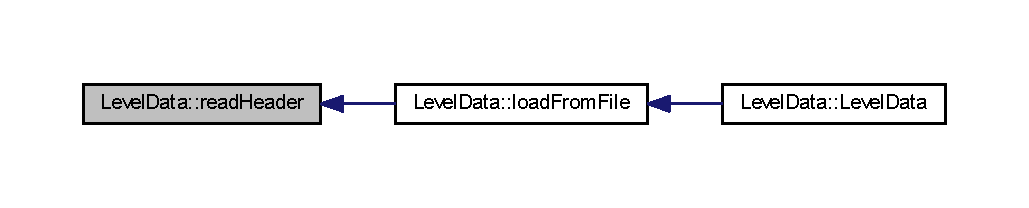
\includegraphics[width=350pt]{classLevelData_a68e8ac8397ac430ebd28f3db2cd2020a_icgraph}
\end{center}
\end{figure}


\hypertarget{classLevelData_ad9e4687d526e6b503617338279aabb33}{\index{Level\+Data@{Level\+Data}!read\+Level@{read\+Level}}
\index{read\+Level@{read\+Level}!Level\+Data@{Level\+Data}}
\subsubsection[{read\+Level}]{\setlength{\rightskip}{0pt plus 5cm}void Level\+Data\+::read\+Level (
\begin{DoxyParamCaption}
\item[{std\+::ifstream \&}]{stream}
\end{DoxyParamCaption}
)\hspace{0.3cm}{\ttfamily [private]}}}\label{classLevelData_ad9e4687d526e6b503617338279aabb33}


Reads the tile data of a level from a given stream. Throws exceptions upon errors. 


\begin{DoxyParams}{Parameters}
{\em stream} & An open file stream to read from. \\
\hline
\end{DoxyParams}


Definition at line 139 of file Level\+Data.\+cpp.



Here is the caller graph for this function\+:
\nopagebreak
\begin{figure}[H]
\begin{center}
\leavevmode
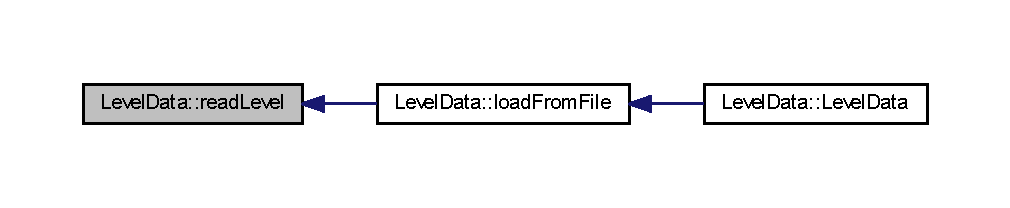
\includegraphics[width=350pt]{classLevelData_ad9e4687d526e6b503617338279aabb33_icgraph}
\end{center}
\end{figure}


\hypertarget{classLevelData_a22aa59bed8da92af1921066eeef30a19}{\index{Level\+Data@{Level\+Data}!determine\+Tile\+Type@{determine\+Tile\+Type}}
\index{determine\+Tile\+Type@{determine\+Tile\+Type}!Level\+Data@{Level\+Data}}
\subsubsection[{determine\+Tile\+Type}]{\setlength{\rightskip}{0pt plus 5cm}{\bf Tile\+Type} Level\+Data\+::determine\+Tile\+Type (
\begin{DoxyParamCaption}
\item[{const char}]{tile}
\end{DoxyParamCaption}
) const\hspace{0.3cm}{\ttfamily [private]}}}\label{classLevelData_a22aa59bed8da92af1921066eeef30a19}


Determines the Tile\+Type which corresponds to the given character. 


\begin{DoxyParams}{Parameters}
{\em tile} & The character which represents a tile value. \\
\hline
\end{DoxyParams}
\begin{DoxyReturn}{Returns}
The correct Tile\+Type, throws an exception if the character is invalid. 
\end{DoxyReturn}


Definition at line 161 of file Level\+Data.\+cpp.



Here is the caller graph for this function\+:
\nopagebreak
\begin{figure}[H]
\begin{center}
\leavevmode
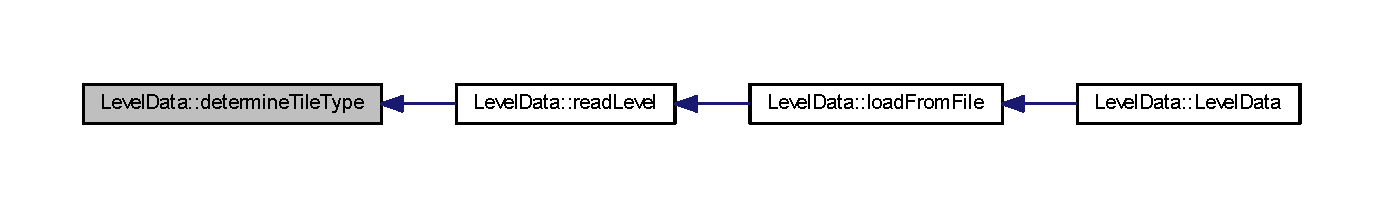
\includegraphics[width=350pt]{classLevelData_a22aa59bed8da92af1921066eeef30a19_icgraph}
\end{center}
\end{figure}




\subsection{Member Data Documentation}
\hypertarget{classLevelData_af2aaac4914ff63edf43f93592e117abf}{\index{Level\+Data@{Level\+Data}!m\+\_\+width@{m\+\_\+width}}
\index{m\+\_\+width@{m\+\_\+width}!Level\+Data@{Level\+Data}}
\subsubsection[{m\+\_\+width}]{\setlength{\rightskip}{0pt plus 5cm}unsigned int Level\+Data\+::m\+\_\+width \{ 0 \}\hspace{0.3cm}{\ttfamily [private]}}}\label{classLevelData_af2aaac4914ff63edf43f93592e117abf}


The number of tiles that make up the level width. 



Definition at line 100 of file Level\+Data.\+hpp.

\hypertarget{classLevelData_af6895162dbf2aae99d81f2bd39bfd0fc}{\index{Level\+Data@{Level\+Data}!m\+\_\+height@{m\+\_\+height}}
\index{m\+\_\+height@{m\+\_\+height}!Level\+Data@{Level\+Data}}
\subsubsection[{m\+\_\+height}]{\setlength{\rightskip}{0pt plus 5cm}unsigned int Level\+Data\+::m\+\_\+height \{ 0 \}\hspace{0.3cm}{\ttfamily [private]}}}\label{classLevelData_af6895162dbf2aae99d81f2bd39bfd0fc}


The number of tiles that make up the level height. 



Definition at line 101 of file Level\+Data.\+hpp.

\hypertarget{classLevelData_a65e6372aea8e8d29fe9a554653a1ad24}{\index{Level\+Data@{Level\+Data}!m\+\_\+map\+File@{m\+\_\+map\+File}}
\index{m\+\_\+map\+File@{m\+\_\+map\+File}!Level\+Data@{Level\+Data}}
\subsubsection[{m\+\_\+map\+File}]{\setlength{\rightskip}{0pt plus 5cm}std\+::string Level\+Data\+::m\+\_\+map\+File = \char`\"{}\char`\"{}\hspace{0.3cm}{\ttfamily [private]}}}\label{classLevelData_a65e6372aea8e8d29fe9a554653a1ad24}


The file location where the level data was loaded from. 



Definition at line 103 of file Level\+Data.\+hpp.

\hypertarget{classLevelData_a32b98877ba76059d320053f55dd97051}{\index{Level\+Data@{Level\+Data}!m\+\_\+tile\+Data@{m\+\_\+tile\+Data}}
\index{m\+\_\+tile\+Data@{m\+\_\+tile\+Data}!Level\+Data@{Level\+Data}}
\subsubsection[{m\+\_\+tile\+Data}]{\setlength{\rightskip}{0pt plus 5cm}std\+::vector$<${\bf Tile\+Type}$>$ Level\+Data\+::m\+\_\+tile\+Data \{ \}\hspace{0.3cm}{\ttfamily [private]}}}\label{classLevelData_a32b98877ba76059d320053f55dd97051}


The type of every tile on the level. 



Definition at line 104 of file Level\+Data.\+hpp.



The documentation for this class was generated from the following files\+:\begin{DoxyCompactItemize}
\item 
U\+:/\+Work/\+Year2/\+G\+E\+C/\+A\+I/\+Source/\+Level/\hyperlink{LevelData_8hpp}{Level\+Data.\+hpp}\item 
U\+:/\+Work/\+Year2/\+G\+E\+C/\+A\+I/\+Source/\+Level/\hyperlink{LevelData_8cpp}{Level\+Data.\+cpp}\end{DoxyCompactItemize}

\hypertarget{classLevelViewer}{\section{Level\+Viewer Class Reference}
\label{classLevelViewer}\index{Level\+Viewer@{Level\+Viewer}}
}


A class used to display the contents of a \hyperlink{classLevelData}{Level\+Data} object on screen.  




{\ttfamily \#include $<$Level\+Viewer.\+hpp$>$}

\subsection*{Public Member Functions}
\begin{DoxyCompactItemize}
\item 
\hyperlink{classLevelViewer_a9455a951428ef99355e4b2431030cabc}{Level\+Viewer} (const \hyperlink{classLevelData}{Level\+Data} \&data)
\begin{DoxyCompactList}\small\item\em Creates a \hyperlink{classLevelViewer}{Level\+Viewer} object from the data contained in the given \hyperlink{classLevelData}{Level\+Data} object. \end{DoxyCompactList}\item 
\hyperlink{classLevelViewer_a6e93342a85445cbebe384e3320317c40}{Level\+Viewer} (\hyperlink{classLevelViewer}{Level\+Viewer} \&\&move)
\item 
\hyperlink{classLevelViewer}{Level\+Viewer} \& \hyperlink{classLevelViewer_aade4f376c18dc077ee4d0ff3112ef18b}{operator=} (\hyperlink{classLevelViewer}{Level\+Viewer} \&\&move)
\item 
\hyperlink{classLevelViewer_a2f53a7ddb76a94061cf4ea426c507791}{Level\+Viewer} (const \hyperlink{classLevelViewer}{Level\+Viewer} \&copy)=default
\item 
\hyperlink{classLevelViewer}{Level\+Viewer} \& \hyperlink{classLevelViewer_aa132fbf52763ffdd77bfcd38335056b8}{operator=} (const \hyperlink{classLevelViewer}{Level\+Viewer} \&copy)=default
\item 
\hyperlink{classLevelViewer_afeecb0c6e492d50e49bc13995b713055}{$\sim$\+Level\+Viewer} ()=default
\item 
const sf\+::\+Texture \& \hyperlink{classLevelViewer_ac7639fd457c73c851c8b86c11a7e7ea1}{get\+View} () const 
\begin{DoxyCompactList}\small\item\em Gets the visual representation of the given \hyperlink{classLevelData}{Level\+Data} object. \end{DoxyCompactList}\item 
const sf\+::\+Vector2f \hyperlink{classLevelViewer_a14f5f87a2bd1169ad44b83cc01c890d3}{get\+Scale} () const 
\begin{DoxyCompactList}\small\item\em Gets the scalar used when drawing the \hyperlink{classLevelData}{Level\+Data} visually. \end{DoxyCompactList}\item 
void \hyperlink{classLevelViewer_a8b6f7c3c274f04b91b9005e51c7325ef}{set\+Scale} (const sf\+::\+Vector2f \&scale)
\begin{DoxyCompactList}\small\item\em Sets the scalar used when drawing the \hyperlink{classLevelData}{Level\+Data} visually. \end{DoxyCompactList}\item 
void \hyperlink{classLevelViewer_a09531b36a9fcc93cd3e2674da74ddd15}{create\+View} (const \hyperlink{classLevelData}{Level\+Data} \&data)
\begin{DoxyCompactList}\small\item\em Creates a representation for the given \hyperlink{classLevelData}{Level\+Data} object. \end{DoxyCompactList}\item 
sf\+::\+Color \hyperlink{classLevelViewer_a86cad499fe0b7978969dd8ba9cbb311f}{determine\+Colour} (const \hyperlink{LevelData_8hpp_a47dee72188473c57343127b1a5843398}{Tile\+Type} tile) const 
\begin{DoxyCompactList}\small\item\em Determines the colour to use based on the given tile. \end{DoxyCompactList}\item 
void \hyperlink{classLevelViewer_a8db6d8e5a3239dc83260c31c047e9d5b}{draw} (sf\+::\+Render\+Target \&draw\+To)
\begin{DoxyCompactList}\small\item\em Causes the \hyperlink{classLevelViewer}{Level\+Viewer} to render itself to a given target. \end{DoxyCompactList}\end{DoxyCompactItemize}
\subsection*{Private Attributes}
\begin{DoxyCompactItemize}
\item 
sf\+::\+Texture \hyperlink{classLevelViewer_a21afdfc2bfc80328897725b1cb911b15}{m\+\_\+view} \{ \}
\begin{DoxyCompactList}\small\item\em The visual representation of the given \hyperlink{classLevelData}{Level\+Data} object. \end{DoxyCompactList}\item 
sf\+::\+Vector2f \hyperlink{classLevelViewer_a1b51d762bb2f7d1917e41bb82d21e90a}{m\+\_\+scale} \{ 1, 1 \}
\begin{DoxyCompactList}\small\item\em The scale to use when displaying the \hyperlink{classLevelData}{Level\+Data} object. \end{DoxyCompactList}\end{DoxyCompactItemize}


\subsection{Detailed Description}
A class used to display the contents of a \hyperlink{classLevelData}{Level\+Data} object on screen. 



Definition at line 17 of file Level\+Viewer.\+hpp.



\subsection{Constructor \& Destructor Documentation}
\hypertarget{classLevelViewer_a9455a951428ef99355e4b2431030cabc}{\index{Level\+Viewer@{Level\+Viewer}!Level\+Viewer@{Level\+Viewer}}
\index{Level\+Viewer@{Level\+Viewer}!Level\+Viewer@{Level\+Viewer}}
\subsubsection[{Level\+Viewer}]{\setlength{\rightskip}{0pt plus 5cm}Level\+Viewer\+::\+Level\+Viewer (
\begin{DoxyParamCaption}
\item[{const {\bf Level\+Data} \&}]{data}
\end{DoxyParamCaption}
)}}\label{classLevelViewer_a9455a951428ef99355e4b2431030cabc}


Creates a \hyperlink{classLevelViewer}{Level\+Viewer} object from the data contained in the given \hyperlink{classLevelData}{Level\+Data} object. 


\begin{DoxyParams}{Parameters}
{\em data} & Contains the data required to produce a visual representation. \\
\hline
\end{DoxyParams}


Definition at line 18 of file Level\+Viewer.\+cpp.

\hypertarget{classLevelViewer_a6e93342a85445cbebe384e3320317c40}{\index{Level\+Viewer@{Level\+Viewer}!Level\+Viewer@{Level\+Viewer}}
\index{Level\+Viewer@{Level\+Viewer}!Level\+Viewer@{Level\+Viewer}}
\subsubsection[{Level\+Viewer}]{\setlength{\rightskip}{0pt plus 5cm}Level\+Viewer\+::\+Level\+Viewer (
\begin{DoxyParamCaption}
\item[{{\bf Level\+Viewer} \&\&}]{move}
\end{DoxyParamCaption}
)}}\label{classLevelViewer_a6e93342a85445cbebe384e3320317c40}


Definition at line 24 of file Level\+Viewer.\+cpp.

\hypertarget{classLevelViewer_a2f53a7ddb76a94061cf4ea426c507791}{\index{Level\+Viewer@{Level\+Viewer}!Level\+Viewer@{Level\+Viewer}}
\index{Level\+Viewer@{Level\+Viewer}!Level\+Viewer@{Level\+Viewer}}
\subsubsection[{Level\+Viewer}]{\setlength{\rightskip}{0pt plus 5cm}Level\+Viewer\+::\+Level\+Viewer (
\begin{DoxyParamCaption}
\item[{const {\bf Level\+Viewer} \&}]{copy}
\end{DoxyParamCaption}
)\hspace{0.3cm}{\ttfamily [default]}}}\label{classLevelViewer_a2f53a7ddb76a94061cf4ea426c507791}
\hypertarget{classLevelViewer_afeecb0c6e492d50e49bc13995b713055}{\index{Level\+Viewer@{Level\+Viewer}!````~Level\+Viewer@{$\sim$\+Level\+Viewer}}
\index{````~Level\+Viewer@{$\sim$\+Level\+Viewer}!Level\+Viewer@{Level\+Viewer}}
\subsubsection[{$\sim$\+Level\+Viewer}]{\setlength{\rightskip}{0pt plus 5cm}Level\+Viewer\+::$\sim$\+Level\+Viewer (
\begin{DoxyParamCaption}
{}
\end{DoxyParamCaption}
)\hspace{0.3cm}{\ttfamily [default]}}}\label{classLevelViewer_afeecb0c6e492d50e49bc13995b713055}


\subsection{Member Function Documentation}
\hypertarget{classLevelViewer_aade4f376c18dc077ee4d0ff3112ef18b}{\index{Level\+Viewer@{Level\+Viewer}!operator=@{operator=}}
\index{operator=@{operator=}!Level\+Viewer@{Level\+Viewer}}
\subsubsection[{operator=}]{\setlength{\rightskip}{0pt plus 5cm}{\bf Level\+Viewer} \& Level\+Viewer\+::operator= (
\begin{DoxyParamCaption}
\item[{{\bf Level\+Viewer} \&\&}]{move}
\end{DoxyParamCaption}
)}}\label{classLevelViewer_aade4f376c18dc077ee4d0ff3112ef18b}


Definition at line 30 of file Level\+Viewer.\+cpp.

\hypertarget{classLevelViewer_aa132fbf52763ffdd77bfcd38335056b8}{\index{Level\+Viewer@{Level\+Viewer}!operator=@{operator=}}
\index{operator=@{operator=}!Level\+Viewer@{Level\+Viewer}}
\subsubsection[{operator=}]{\setlength{\rightskip}{0pt plus 5cm}{\bf Level\+Viewer}\& Level\+Viewer\+::operator= (
\begin{DoxyParamCaption}
\item[{const {\bf Level\+Viewer} \&}]{copy}
\end{DoxyParamCaption}
)\hspace{0.3cm}{\ttfamily [default]}}}\label{classLevelViewer_aa132fbf52763ffdd77bfcd38335056b8}
\hypertarget{classLevelViewer_ac7639fd457c73c851c8b86c11a7e7ea1}{\index{Level\+Viewer@{Level\+Viewer}!get\+View@{get\+View}}
\index{get\+View@{get\+View}!Level\+Viewer@{Level\+Viewer}}
\subsubsection[{get\+View}]{\setlength{\rightskip}{0pt plus 5cm}const sf\+::\+Texture\& Level\+Viewer\+::get\+View (
\begin{DoxyParamCaption}
{}
\end{DoxyParamCaption}
) const\hspace{0.3cm}{\ttfamily [inline]}}}\label{classLevelViewer_ac7639fd457c73c851c8b86c11a7e7ea1}


Gets the visual representation of the given \hyperlink{classLevelData}{Level\+Data} object. 



Definition at line 42 of file Level\+Viewer.\+hpp.

\hypertarget{classLevelViewer_a14f5f87a2bd1169ad44b83cc01c890d3}{\index{Level\+Viewer@{Level\+Viewer}!get\+Scale@{get\+Scale}}
\index{get\+Scale@{get\+Scale}!Level\+Viewer@{Level\+Viewer}}
\subsubsection[{get\+Scale}]{\setlength{\rightskip}{0pt plus 5cm}const sf\+::\+Vector2f Level\+Viewer\+::get\+Scale (
\begin{DoxyParamCaption}
{}
\end{DoxyParamCaption}
) const\hspace{0.3cm}{\ttfamily [inline]}}}\label{classLevelViewer_a14f5f87a2bd1169ad44b83cc01c890d3}


Gets the scalar used when drawing the \hyperlink{classLevelData}{Level\+Data} visually. 



Definition at line 45 of file Level\+Viewer.\+hpp.

\hypertarget{classLevelViewer_a8b6f7c3c274f04b91b9005e51c7325ef}{\index{Level\+Viewer@{Level\+Viewer}!set\+Scale@{set\+Scale}}
\index{set\+Scale@{set\+Scale}!Level\+Viewer@{Level\+Viewer}}
\subsubsection[{set\+Scale}]{\setlength{\rightskip}{0pt plus 5cm}void Level\+Viewer\+::set\+Scale (
\begin{DoxyParamCaption}
\item[{const sf\+::\+Vector2f \&}]{scale}
\end{DoxyParamCaption}
)\hspace{0.3cm}{\ttfamily [inline]}}}\label{classLevelViewer_a8b6f7c3c274f04b91b9005e51c7325ef}


Sets the scalar used when drawing the \hyperlink{classLevelData}{Level\+Data} visually. 


\begin{DoxyParams}{Parameters}
{\em scale} & The new scale values. \\
\hline
\end{DoxyParams}


Definition at line 49 of file Level\+Viewer.\+hpp.

\hypertarget{classLevelViewer_a09531b36a9fcc93cd3e2674da74ddd15}{\index{Level\+Viewer@{Level\+Viewer}!create\+View@{create\+View}}
\index{create\+View@{create\+View}!Level\+Viewer@{Level\+Viewer}}
\subsubsection[{create\+View}]{\setlength{\rightskip}{0pt plus 5cm}void Level\+Viewer\+::create\+View (
\begin{DoxyParamCaption}
\item[{const {\bf Level\+Data} \&}]{data}
\end{DoxyParamCaption}
)}}\label{classLevelViewer_a09531b36a9fcc93cd3e2674da74ddd15}


Creates a representation for the given \hyperlink{classLevelData}{Level\+Data} object. 


\begin{DoxyParams}{Parameters}
{\em data} & The data to create a visualisation for. \\
\hline
\end{DoxyParams}


Definition at line 47 of file Level\+Viewer.\+cpp.



Here is the caller graph for this function\+:
\nopagebreak
\begin{figure}[H]
\begin{center}
\leavevmode
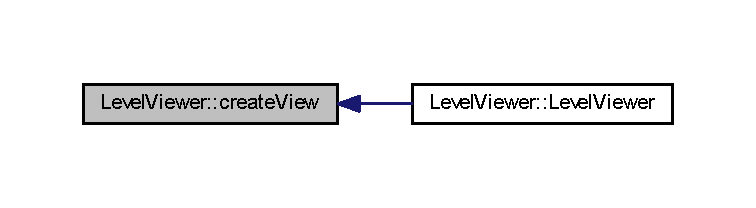
\includegraphics[width=350pt]{classLevelViewer_a09531b36a9fcc93cd3e2674da74ddd15_icgraph}
\end{center}
\end{figure}


\hypertarget{classLevelViewer_a86cad499fe0b7978969dd8ba9cbb311f}{\index{Level\+Viewer@{Level\+Viewer}!determine\+Colour@{determine\+Colour}}
\index{determine\+Colour@{determine\+Colour}!Level\+Viewer@{Level\+Viewer}}
\subsubsection[{determine\+Colour}]{\setlength{\rightskip}{0pt plus 5cm}sf\+::\+Color Level\+Viewer\+::determine\+Colour (
\begin{DoxyParamCaption}
\item[{const {\bf Tile\+Type}}]{tile}
\end{DoxyParamCaption}
) const}}\label{classLevelViewer_a86cad499fe0b7978969dd8ba9cbb311f}


Determines the colour to use based on the given tile. 


\begin{DoxyParams}{Parameters}
{\em tile} & The tile to retrieve the colour for. \\
\hline
\end{DoxyParams}
\begin{DoxyReturn}{Returns}
A colour value. 
\end{DoxyReturn}


Definition at line 72 of file Level\+Viewer.\+cpp.



Here is the caller graph for this function\+:
\nopagebreak
\begin{figure}[H]
\begin{center}
\leavevmode
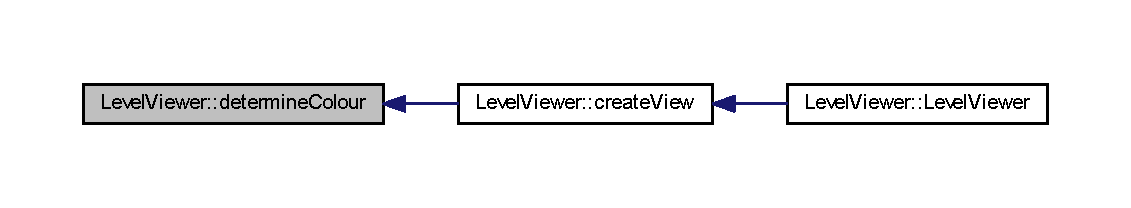
\includegraphics[width=350pt]{classLevelViewer_a86cad499fe0b7978969dd8ba9cbb311f_icgraph}
\end{center}
\end{figure}


\hypertarget{classLevelViewer_a8db6d8e5a3239dc83260c31c047e9d5b}{\index{Level\+Viewer@{Level\+Viewer}!draw@{draw}}
\index{draw@{draw}!Level\+Viewer@{Level\+Viewer}}
\subsubsection[{draw}]{\setlength{\rightskip}{0pt plus 5cm}void Level\+Viewer\+::draw (
\begin{DoxyParamCaption}
\item[{sf\+::\+Render\+Target \&}]{draw\+To}
\end{DoxyParamCaption}
)}}\label{classLevelViewer_a8db6d8e5a3239dc83260c31c047e9d5b}


Causes the \hyperlink{classLevelViewer}{Level\+Viewer} to render itself to a given target. 


\begin{DoxyParams}{Parameters}
{\em draw\+To} & The object to draw onto. \\
\hline
\end{DoxyParams}


Definition at line 108 of file Level\+Viewer.\+cpp.



\subsection{Member Data Documentation}
\hypertarget{classLevelViewer_a21afdfc2bfc80328897725b1cb911b15}{\index{Level\+Viewer@{Level\+Viewer}!m\+\_\+view@{m\+\_\+view}}
\index{m\+\_\+view@{m\+\_\+view}!Level\+Viewer@{Level\+Viewer}}
\subsubsection[{m\+\_\+view}]{\setlength{\rightskip}{0pt plus 5cm}sf\+::\+Texture Level\+Viewer\+::m\+\_\+view \{ \}\hspace{0.3cm}{\ttfamily [private]}}}\label{classLevelViewer_a21afdfc2bfc80328897725b1cb911b15}


The visual representation of the given \hyperlink{classLevelData}{Level\+Data} object. 



Definition at line 75 of file Level\+Viewer.\+hpp.

\hypertarget{classLevelViewer_a1b51d762bb2f7d1917e41bb82d21e90a}{\index{Level\+Viewer@{Level\+Viewer}!m\+\_\+scale@{m\+\_\+scale}}
\index{m\+\_\+scale@{m\+\_\+scale}!Level\+Viewer@{Level\+Viewer}}
\subsubsection[{m\+\_\+scale}]{\setlength{\rightskip}{0pt plus 5cm}sf\+::\+Vector2f Level\+Viewer\+::m\+\_\+scale \{ 1, 1 \}\hspace{0.3cm}{\ttfamily [private]}}}\label{classLevelViewer_a1b51d762bb2f7d1917e41bb82d21e90a}


The scale to use when displaying the \hyperlink{classLevelData}{Level\+Data} object. 



Definition at line 76 of file Level\+Viewer.\+hpp.



The documentation for this class was generated from the following files\+:\begin{DoxyCompactItemize}
\item 
U\+:/\+Work/\+Year2/\+G\+E\+C/\+A\+I/\+Source/\+Level/\hyperlink{LevelViewer_8hpp}{Level\+Viewer.\+hpp}\item 
U\+:/\+Work/\+Year2/\+G\+E\+C/\+A\+I/\+Source/\+Level/\hyperlink{LevelViewer_8cpp}{Level\+Viewer.\+cpp}\end{DoxyCompactItemize}

\hypertarget{classRRT}{\section{R\+R\+T Class Reference}
\label{classRRT}\index{R\+R\+T@{R\+R\+T}}
}


A class which creates an \hyperlink{classRRT}{R\+R\+T} tree when given a map and a start and end point.  




{\ttfamily \#include $<$R\+R\+T.\+hpp$>$}

\subsection*{Public Member Functions}
\begin{DoxyCompactItemize}
\item 
\hyperlink{classRRT_ab5a2cf5a9d8adb4077034047b7764c1b}{R\+R\+T} (const float sample\+Distance=0.\+25f, const float branch\+Distance=15.\+f)
\begin{DoxyCompactList}\small\item\em Construct an \hyperlink{classRRT}{R\+R\+T} object with the required algorithm parameters. \end{DoxyCompactList}\item 
\hyperlink{classRRT_ad5ead60ff7ffe318629226ee130d3e71}{R\+R\+T} (\hyperlink{classRRT}{R\+R\+T} \&\&move)
\item 
\hyperlink{classRRT}{R\+R\+T} \& \hyperlink{classRRT_ac93c18af76ce7b91b981daeac72146ce}{operator=} (\hyperlink{classRRT}{R\+R\+T} \&\&move)
\item 
\hyperlink{classRRT_a3636453ca77a4c95f0a9d0efffde30f7}{R\+R\+T} (const \hyperlink{classRRT}{R\+R\+T} \&copy)=default
\item 
\hyperlink{classRRT}{R\+R\+T} \& \hyperlink{classRRT_a94b62c34f8ada82dc56c620fdaf0a13c}{operator=} (const \hyperlink{classRRT}{R\+R\+T} \&copy)=default
\item 
\hyperlink{classRRT_af5f26f011cc50d90f7e93d6cd297920c}{$\sim$\+R\+R\+T} ()=default
\item 
const sf\+::\+Vector2i \& \hyperlink{classRRT_ad3cf3f119687f64b14ad5234daae3dc5}{get\+Start} () const 
\begin{DoxyCompactList}\small\item\em Obtains the starting point of the \hyperlink{classRRT}{R\+R\+T} algorithm. \end{DoxyCompactList}\item 
const sf\+::\+Vector2i \& \hyperlink{classRRT_a320e5980cb9a3a8e4a422b03bff1da73}{get\+End} () const 
\begin{DoxyCompactList}\small\item\em Obtains the end point of the \hyperlink{classRRT}{R\+R\+T} algorithm. \end{DoxyCompactList}\item 
void \hyperlink{classRRT_ace95930cd4860fc4afb9ccc329e1f010}{draw} (sf\+::\+Render\+Target \&draw\+To, const sf\+::\+Vector2f \&scale)
\begin{DoxyCompactList}\small\item\em Draws the entire \hyperlink{classRRT}{R\+R\+T} tree to the given target. \end{DoxyCompactList}\item 
bool \hyperlink{classRRT_a9b27ef76b0e43d8ff3f10ed9db287c35}{has\+Finished} () const 
\begin{DoxyCompactList}\small\item\em Determines if the goal has been reached. \end{DoxyCompactList}\item 
void \hyperlink{classRRT_ab874a1061b18086df06ac1e4dc91b27d}{prepare\+Tree} (const std\+::shared\+\_\+ptr$<$ \hyperlink{classLevelData}{Level\+Data} $>$ \&data, const sf\+::\+Vector2i \&start, const sf\+::\+Vector2i \&end)
\begin{DoxyCompactList}\small\item\em Prepares the \hyperlink{classRRT}{R\+R\+T} algorithm for generating nodes. \end{DoxyCompactList}\item 
void \hyperlink{classRRT_ad906dded9e6d3bb3f1f1f5972cd3fdf7}{generate\+Branch} ()
\begin{DoxyCompactList}\small\item\em Causes the algorithm to produce an extra branch if it hasn't already reached the goal. \end{DoxyCompactList}\item 
bool \hyperlink{classRRT_ac87ec16ecb94d25a9941b29c75dc83fa}{is\+Valid\+Tile} (const sf\+::\+Vector2i \&position, const \hyperlink{LevelData_8hpp_a47dee72188473c57343127b1a5843398}{Tile\+Type} base) const 
\begin{DoxyCompactList}\small\item\em Checks if the tile at the given position is valid according to the base type. \end{DoxyCompactList}\end{DoxyCompactItemize}
\subsection*{Private Member Functions}
\begin{DoxyCompactItemize}
\item 
R\+R\+T\+Tree\+::\+Branch \hyperlink{classRRT_a21ff259bb7d646a09667b50602663abf}{determine\+Nearest} (const sf\+::\+Vector2i \&position) const 
\begin{DoxyCompactList}\small\item\em Determines the Branch closest to the given position. \end{DoxyCompactList}\item 
R\+R\+T\+Tree\+::\+Branch \hyperlink{classRRT_a1393c4dc3be5c4d66756dbfb8b75abee}{calculate\+Branch} (const sf\+::\+Vector2i \&start, const sf\+::\+Vector2i \&end) const 
\begin{DoxyCompactList}\small\item\em Calculates a new branch between the start and end point by sampling and checking for collision. \end{DoxyCompactList}\end{DoxyCompactItemize}
\subsection*{Private Attributes}
\begin{DoxyCompactItemize}
\item 
std\+::shared\+\_\+ptr$<$ \hyperlink{classLevelData}{Level\+Data} $>$ \hyperlink{classRRT_a4990cccae7cd2160f1fa6e970242365a}{m\+\_\+data} \{ \}
\begin{DoxyCompactList}\small\item\em A pointer to the \hyperlink{classLevelData}{Level\+Data} which the \hyperlink{classTree}{Tree} will be generated with. \end{DoxyCompactList}\item 
sf\+::\+Vector2i \hyperlink{classRRT_a4f0394ed9f6cd596f13b19a1617e56f9}{m\+\_\+start} \{ \}
\begin{DoxyCompactList}\small\item\em The start point of the \hyperlink{classRRT}{R\+R\+T} algorithm. \end{DoxyCompactList}\item 
sf\+::\+Vector2i \hyperlink{classRRT_a96f886227de84066adb285cbc6dcb2f5}{m\+\_\+end} \{ \}
\begin{DoxyCompactList}\small\item\em The end point of the \hyperlink{classRRT}{R\+R\+T} algorithm. \end{DoxyCompactList}\item 
float \hyperlink{classRRT_ad1501f1319a73e96ebdc3a9bb76dbdca}{m\+\_\+sample\+Distance} \{ 0 \}
\begin{DoxyCompactList}\small\item\em How much to increment by when sampling the distance. \end{DoxyCompactList}\item 
float \hyperlink{classRRT_a2aaaa69617cfd685ae1d504e3cf31317}{m\+\_\+branch\+Distance} \{ 0 \}
\begin{DoxyCompactList}\small\item\em The maximum distance of a branch. \end{DoxyCompactList}\item 
std\+::vector$<$ R\+R\+T\+Tree\+::\+Branch $>$ \hyperlink{classRRT_a25e924b6450a7dc97c4ecff2735b5889}{m\+\_\+nodes} \{ \}
\begin{DoxyCompactList}\small\item\em A collection of pointers to each branch in tile order. \end{DoxyCompactList}\item 
std\+::shared\+\_\+ptr$<$ \hyperlink{RRT_8hpp_ad96bf2a5632cc2b01900b403e90b1607}{R\+R\+T\+Tree} $>$ \hyperlink{classRRT_a2905ea09c16ae59d6ee1beae15d12b2e}{m\+\_\+tree} \{ \}
\begin{DoxyCompactList}\small\item\em The tree containing each node and its branches. \end{DoxyCompactList}\end{DoxyCompactItemize}


\subsection{Detailed Description}
A class which creates an \hyperlink{classRRT}{R\+R\+T} tree when given a map and a start and end point. 



Definition at line 27 of file R\+R\+T.\+hpp.



\subsection{Constructor \& Destructor Documentation}
\hypertarget{classRRT_ab5a2cf5a9d8adb4077034047b7764c1b}{\index{R\+R\+T@{R\+R\+T}!R\+R\+T@{R\+R\+T}}
\index{R\+R\+T@{R\+R\+T}!R\+R\+T@{R\+R\+T}}
\subsubsection[{R\+R\+T}]{\setlength{\rightskip}{0pt plus 5cm}R\+R\+T\+::\+R\+R\+T (
\begin{DoxyParamCaption}
\item[{const float}]{sample\+Distance = {\ttfamily 0.25f}, }
\item[{const float}]{branch\+Distance = {\ttfamily 15.f}}
\end{DoxyParamCaption}
)}}\label{classRRT_ab5a2cf5a9d8adb4077034047b7764c1b}


Construct an \hyperlink{classRRT}{R\+R\+T} object with the required algorithm parameters. 


\begin{DoxyParams}{Parameters}
{\em sample\+Distance} & The incrementation to use when sampling between branches during collision detection. \\
\hline
{\em branch\+Distance} & The maximum distance of a branch. \\
\hline
\end{DoxyParams}


Definition at line 21 of file R\+R\+T.\+cpp.

\hypertarget{classRRT_ad5ead60ff7ffe318629226ee130d3e71}{\index{R\+R\+T@{R\+R\+T}!R\+R\+T@{R\+R\+T}}
\index{R\+R\+T@{R\+R\+T}!R\+R\+T@{R\+R\+T}}
\subsubsection[{R\+R\+T}]{\setlength{\rightskip}{0pt plus 5cm}R\+R\+T\+::\+R\+R\+T (
\begin{DoxyParamCaption}
\item[{{\bf R\+R\+T} \&\&}]{move}
\end{DoxyParamCaption}
)}}\label{classRRT_ad5ead60ff7ffe318629226ee130d3e71}


Definition at line 31 of file R\+R\+T.\+cpp.

\hypertarget{classRRT_a3636453ca77a4c95f0a9d0efffde30f7}{\index{R\+R\+T@{R\+R\+T}!R\+R\+T@{R\+R\+T}}
\index{R\+R\+T@{R\+R\+T}!R\+R\+T@{R\+R\+T}}
\subsubsection[{R\+R\+T}]{\setlength{\rightskip}{0pt plus 5cm}R\+R\+T\+::\+R\+R\+T (
\begin{DoxyParamCaption}
\item[{const {\bf R\+R\+T} \&}]{copy}
\end{DoxyParamCaption}
)\hspace{0.3cm}{\ttfamily [default]}}}\label{classRRT_a3636453ca77a4c95f0a9d0efffde30f7}
\hypertarget{classRRT_af5f26f011cc50d90f7e93d6cd297920c}{\index{R\+R\+T@{R\+R\+T}!````~R\+R\+T@{$\sim$\+R\+R\+T}}
\index{````~R\+R\+T@{$\sim$\+R\+R\+T}!R\+R\+T@{R\+R\+T}}
\subsubsection[{$\sim$\+R\+R\+T}]{\setlength{\rightskip}{0pt plus 5cm}R\+R\+T\+::$\sim$\+R\+R\+T (
\begin{DoxyParamCaption}
{}
\end{DoxyParamCaption}
)\hspace{0.3cm}{\ttfamily [default]}}}\label{classRRT_af5f26f011cc50d90f7e93d6cd297920c}


\subsection{Member Function Documentation}
\hypertarget{classRRT_ac93c18af76ce7b91b981daeac72146ce}{\index{R\+R\+T@{R\+R\+T}!operator=@{operator=}}
\index{operator=@{operator=}!R\+R\+T@{R\+R\+T}}
\subsubsection[{operator=}]{\setlength{\rightskip}{0pt plus 5cm}{\bf R\+R\+T} \& R\+R\+T\+::operator= (
\begin{DoxyParamCaption}
\item[{{\bf R\+R\+T} \&\&}]{move}
\end{DoxyParamCaption}
)}}\label{classRRT_ac93c18af76ce7b91b981daeac72146ce}


Definition at line 37 of file R\+R\+T.\+cpp.

\hypertarget{classRRT_a94b62c34f8ada82dc56c620fdaf0a13c}{\index{R\+R\+T@{R\+R\+T}!operator=@{operator=}}
\index{operator=@{operator=}!R\+R\+T@{R\+R\+T}}
\subsubsection[{operator=}]{\setlength{\rightskip}{0pt plus 5cm}{\bf R\+R\+T}\& R\+R\+T\+::operator= (
\begin{DoxyParamCaption}
\item[{const {\bf R\+R\+T} \&}]{copy}
\end{DoxyParamCaption}
)\hspace{0.3cm}{\ttfamily [default]}}}\label{classRRT_a94b62c34f8ada82dc56c620fdaf0a13c}
\hypertarget{classRRT_ad3cf3f119687f64b14ad5234daae3dc5}{\index{R\+R\+T@{R\+R\+T}!get\+Start@{get\+Start}}
\index{get\+Start@{get\+Start}!R\+R\+T@{R\+R\+T}}
\subsubsection[{get\+Start}]{\setlength{\rightskip}{0pt plus 5cm}const sf\+::\+Vector2i\& R\+R\+T\+::get\+Start (
\begin{DoxyParamCaption}
{}
\end{DoxyParamCaption}
) const\hspace{0.3cm}{\ttfamily [inline]}}}\label{classRRT_ad3cf3f119687f64b14ad5234daae3dc5}


Obtains the starting point of the \hyperlink{classRRT}{R\+R\+T} algorithm. 



Definition at line 53 of file R\+R\+T.\+hpp.

\hypertarget{classRRT_a320e5980cb9a3a8e4a422b03bff1da73}{\index{R\+R\+T@{R\+R\+T}!get\+End@{get\+End}}
\index{get\+End@{get\+End}!R\+R\+T@{R\+R\+T}}
\subsubsection[{get\+End}]{\setlength{\rightskip}{0pt plus 5cm}const sf\+::\+Vector2i\& R\+R\+T\+::get\+End (
\begin{DoxyParamCaption}
{}
\end{DoxyParamCaption}
) const\hspace{0.3cm}{\ttfamily [inline]}}}\label{classRRT_a320e5980cb9a3a8e4a422b03bff1da73}


Obtains the end point of the \hyperlink{classRRT}{R\+R\+T} algorithm. 



Definition at line 56 of file R\+R\+T.\+hpp.

\hypertarget{classRRT_ace95930cd4860fc4afb9ccc329e1f010}{\index{R\+R\+T@{R\+R\+T}!draw@{draw}}
\index{draw@{draw}!R\+R\+T@{R\+R\+T}}
\subsubsection[{draw}]{\setlength{\rightskip}{0pt plus 5cm}void R\+R\+T\+::draw (
\begin{DoxyParamCaption}
\item[{sf\+::\+Render\+Target \&}]{draw\+To, }
\item[{const sf\+::\+Vector2f \&}]{scale}
\end{DoxyParamCaption}
)}}\label{classRRT_ace95930cd4860fc4afb9ccc329e1f010}


Draws the entire \hyperlink{classRRT}{R\+R\+T} tree to the given target. 


\begin{DoxyParams}{Parameters}
{\em draw\+To} & The target to draw the tree to. \\
\hline
{\em scale} & The scalar to used when determining pixel position. \\
\hline
\end{DoxyParams}


Definition at line 65 of file R\+R\+T.\+cpp.

\hypertarget{classRRT_a9b27ef76b0e43d8ff3f10ed9db287c35}{\index{R\+R\+T@{R\+R\+T}!has\+Finished@{has\+Finished}}
\index{has\+Finished@{has\+Finished}!R\+R\+T@{R\+R\+T}}
\subsubsection[{has\+Finished}]{\setlength{\rightskip}{0pt plus 5cm}bool R\+R\+T\+::has\+Finished (
\begin{DoxyParamCaption}
{}
\end{DoxyParamCaption}
) const}}\label{classRRT_a9b27ef76b0e43d8ff3f10ed9db287c35}


Determines if the goal has been reached. 



Definition at line 111 of file R\+R\+T.\+cpp.



Here is the caller graph for this function\+:
\nopagebreak
\begin{figure}[H]
\begin{center}
\leavevmode
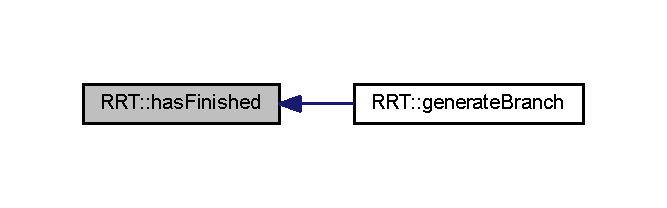
\includegraphics[width=320pt]{classRRT_a9b27ef76b0e43d8ff3f10ed9db287c35_icgraph}
\end{center}
\end{figure}


\hypertarget{classRRT_ab874a1061b18086df06ac1e4dc91b27d}{\index{R\+R\+T@{R\+R\+T}!prepare\+Tree@{prepare\+Tree}}
\index{prepare\+Tree@{prepare\+Tree}!R\+R\+T@{R\+R\+T}}
\subsubsection[{prepare\+Tree}]{\setlength{\rightskip}{0pt plus 5cm}void R\+R\+T\+::prepare\+Tree (
\begin{DoxyParamCaption}
\item[{const std\+::shared\+\_\+ptr$<$ {\bf Level\+Data} $>$ \&}]{data, }
\item[{const sf\+::\+Vector2i \&}]{start, }
\item[{const sf\+::\+Vector2i \&}]{end}
\end{DoxyParamCaption}
)}}\label{classRRT_ab874a1061b18086df06ac1e4dc91b27d}


Prepares the \hyperlink{classRRT}{R\+R\+T} algorithm for generating nodes. 


\begin{DoxyParams}{Parameters}
{\em data} & The data to create a tree from. \\
\hline
{\em start} & The start point of the \hyperlink{classRRT}{R\+R\+T} algorithm. \\
\hline
{\em end} & The end point of the \hyperlink{classRRT}{R\+R\+T} algorithm. \\
\hline
\end{DoxyParams}


Definition at line 125 of file R\+R\+T.\+cpp.

\hypertarget{classRRT_ad906dded9e6d3bb3f1f1f5972cd3fdf7}{\index{R\+R\+T@{R\+R\+T}!generate\+Branch@{generate\+Branch}}
\index{generate\+Branch@{generate\+Branch}!R\+R\+T@{R\+R\+T}}
\subsubsection[{generate\+Branch}]{\setlength{\rightskip}{0pt plus 5cm}void R\+R\+T\+::generate\+Branch (
\begin{DoxyParamCaption}
{}
\end{DoxyParamCaption}
)}}\label{classRRT_ad906dded9e6d3bb3f1f1f5972cd3fdf7}


Causes the algorithm to produce an extra branch if it hasn't already reached the goal. 



Definition at line 150 of file R\+R\+T.\+cpp.

\hypertarget{classRRT_ac87ec16ecb94d25a9941b29c75dc83fa}{\index{R\+R\+T@{R\+R\+T}!is\+Valid\+Tile@{is\+Valid\+Tile}}
\index{is\+Valid\+Tile@{is\+Valid\+Tile}!R\+R\+T@{R\+R\+T}}
\subsubsection[{is\+Valid\+Tile}]{\setlength{\rightskip}{0pt plus 5cm}bool R\+R\+T\+::is\+Valid\+Tile (
\begin{DoxyParamCaption}
\item[{const sf\+::\+Vector2i \&}]{position, }
\item[{const {\bf Tile\+Type}}]{base}
\end{DoxyParamCaption}
) const}}\label{classRRT_ac87ec16ecb94d25a9941b29c75dc83fa}


Checks if the tile at the given position is valid according to the base type. 


\begin{DoxyParams}{Parameters}
{\em position} & The position to check. \\
\hline
{\em base} & The base tile, this impacts whether the tile is valid. \hyperlink{LevelData_8hpp_a47dee72188473c57343127b1a5843398a46dc1018ac1d8fca7c2752a61ce2fd0f}{Tile\+Type\+::\+Out\+Of\+Bounds} allows any tile. \\
\hline
\end{DoxyParams}
\begin{DoxyReturn}{Returns}
A \hyperlink{LevelData_8hpp_a47dee72188473c57343127b1a5843398a27634ff8002b12e75d98e07ccd005d18}{Tile\+Type\+::\+Water} base can only travel on water, the rest can travel on land only. 
\end{DoxyReturn}


Definition at line 195 of file R\+R\+T.\+cpp.



Here is the caller graph for this function\+:
\nopagebreak
\begin{figure}[H]
\begin{center}
\leavevmode
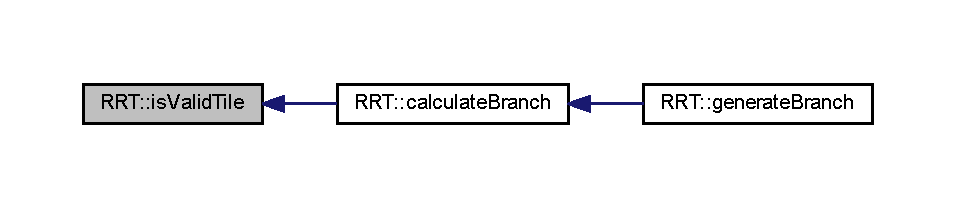
\includegraphics[width=350pt]{classRRT_ac87ec16ecb94d25a9941b29c75dc83fa_icgraph}
\end{center}
\end{figure}


\hypertarget{classRRT_a21ff259bb7d646a09667b50602663abf}{\index{R\+R\+T@{R\+R\+T}!determine\+Nearest@{determine\+Nearest}}
\index{determine\+Nearest@{determine\+Nearest}!R\+R\+T@{R\+R\+T}}
\subsubsection[{determine\+Nearest}]{\setlength{\rightskip}{0pt plus 5cm}R\+R\+T\+Tree\+::\+Branch R\+R\+T\+::determine\+Nearest (
\begin{DoxyParamCaption}
\item[{const sf\+::\+Vector2i \&}]{position}
\end{DoxyParamCaption}
) const\hspace{0.3cm}{\ttfamily [private]}}}\label{classRRT_a21ff259bb7d646a09667b50602663abf}


Determines the Branch closest to the given position. 


\begin{DoxyParams}{Parameters}
{\em position} & The position to check for. \\
\hline
\end{DoxyParams}
\begin{DoxyReturn}{Returns}
The closest Branch. 
\end{DoxyReturn}


Definition at line 215 of file R\+R\+T.\+cpp.



Here is the caller graph for this function\+:
\nopagebreak
\begin{figure}[H]
\begin{center}
\leavevmode
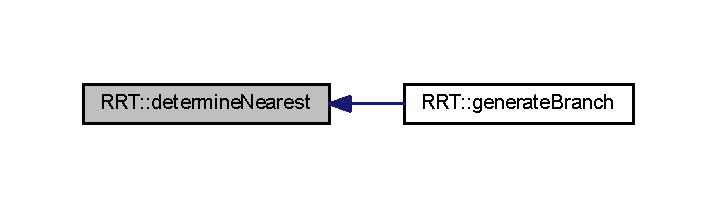
\includegraphics[width=344pt]{classRRT_a21ff259bb7d646a09667b50602663abf_icgraph}
\end{center}
\end{figure}


\hypertarget{classRRT_a1393c4dc3be5c4d66756dbfb8b75abee}{\index{R\+R\+T@{R\+R\+T}!calculate\+Branch@{calculate\+Branch}}
\index{calculate\+Branch@{calculate\+Branch}!R\+R\+T@{R\+R\+T}}
\subsubsection[{calculate\+Branch}]{\setlength{\rightskip}{0pt plus 5cm}R\+R\+T\+Tree\+::\+Branch R\+R\+T\+::calculate\+Branch (
\begin{DoxyParamCaption}
\item[{const sf\+::\+Vector2i \&}]{start, }
\item[{const sf\+::\+Vector2i \&}]{end}
\end{DoxyParamCaption}
) const\hspace{0.3cm}{\ttfamily [private]}}}\label{classRRT_a1393c4dc3be5c4d66756dbfb8b75abee}


Calculates a new branch between the start and end point by sampling and checking for collision. 


\begin{DoxyParams}{Parameters}
{\em start} & The position to start from. \\
\hline
{\em end} & The target position. \\
\hline
\end{DoxyParams}
\begin{DoxyReturn}{Returns}
A new branch, this will be a nullptr if a branch couldn't be generated. 
\end{DoxyReturn}


Definition at line 245 of file R\+R\+T.\+cpp.



Here is the caller graph for this function\+:
\nopagebreak
\begin{figure}[H]
\begin{center}
\leavevmode
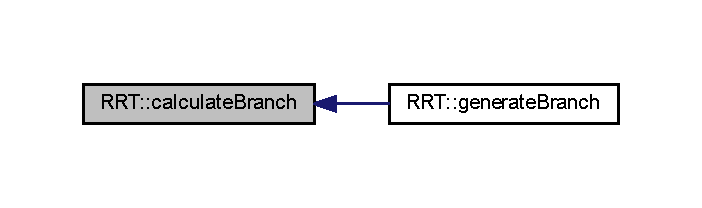
\includegraphics[width=337pt]{classRRT_a1393c4dc3be5c4d66756dbfb8b75abee_icgraph}
\end{center}
\end{figure}




\subsection{Member Data Documentation}
\hypertarget{classRRT_a4990cccae7cd2160f1fa6e970242365a}{\index{R\+R\+T@{R\+R\+T}!m\+\_\+data@{m\+\_\+data}}
\index{m\+\_\+data@{m\+\_\+data}!R\+R\+T@{R\+R\+T}}
\subsubsection[{m\+\_\+data}]{\setlength{\rightskip}{0pt plus 5cm}std\+::shared\+\_\+ptr$<${\bf Level\+Data}$>$ R\+R\+T\+::m\+\_\+data \{ \}\hspace{0.3cm}{\ttfamily [private]}}}\label{classRRT_a4990cccae7cd2160f1fa6e970242365a}


A pointer to the \hyperlink{classLevelData}{Level\+Data} which the \hyperlink{classTree}{Tree} will be generated with. 



Definition at line 109 of file R\+R\+T.\+hpp.

\hypertarget{classRRT_a4f0394ed9f6cd596f13b19a1617e56f9}{\index{R\+R\+T@{R\+R\+T}!m\+\_\+start@{m\+\_\+start}}
\index{m\+\_\+start@{m\+\_\+start}!R\+R\+T@{R\+R\+T}}
\subsubsection[{m\+\_\+start}]{\setlength{\rightskip}{0pt plus 5cm}sf\+::\+Vector2i R\+R\+T\+::m\+\_\+start \{ \}\hspace{0.3cm}{\ttfamily [private]}}}\label{classRRT_a4f0394ed9f6cd596f13b19a1617e56f9}


The start point of the \hyperlink{classRRT}{R\+R\+T} algorithm. 



Definition at line 110 of file R\+R\+T.\+hpp.

\hypertarget{classRRT_a96f886227de84066adb285cbc6dcb2f5}{\index{R\+R\+T@{R\+R\+T}!m\+\_\+end@{m\+\_\+end}}
\index{m\+\_\+end@{m\+\_\+end}!R\+R\+T@{R\+R\+T}}
\subsubsection[{m\+\_\+end}]{\setlength{\rightskip}{0pt plus 5cm}sf\+::\+Vector2i R\+R\+T\+::m\+\_\+end \{ \}\hspace{0.3cm}{\ttfamily [private]}}}\label{classRRT_a96f886227de84066adb285cbc6dcb2f5}


The end point of the \hyperlink{classRRT}{R\+R\+T} algorithm. 



Definition at line 111 of file R\+R\+T.\+hpp.

\hypertarget{classRRT_ad1501f1319a73e96ebdc3a9bb76dbdca}{\index{R\+R\+T@{R\+R\+T}!m\+\_\+sample\+Distance@{m\+\_\+sample\+Distance}}
\index{m\+\_\+sample\+Distance@{m\+\_\+sample\+Distance}!R\+R\+T@{R\+R\+T}}
\subsubsection[{m\+\_\+sample\+Distance}]{\setlength{\rightskip}{0pt plus 5cm}float R\+R\+T\+::m\+\_\+sample\+Distance \{ 0 \}\hspace{0.3cm}{\ttfamily [private]}}}\label{classRRT_ad1501f1319a73e96ebdc3a9bb76dbdca}


How much to increment by when sampling the distance. 



Definition at line 113 of file R\+R\+T.\+hpp.

\hypertarget{classRRT_a2aaaa69617cfd685ae1d504e3cf31317}{\index{R\+R\+T@{R\+R\+T}!m\+\_\+branch\+Distance@{m\+\_\+branch\+Distance}}
\index{m\+\_\+branch\+Distance@{m\+\_\+branch\+Distance}!R\+R\+T@{R\+R\+T}}
\subsubsection[{m\+\_\+branch\+Distance}]{\setlength{\rightskip}{0pt plus 5cm}float R\+R\+T\+::m\+\_\+branch\+Distance \{ 0 \}\hspace{0.3cm}{\ttfamily [private]}}}\label{classRRT_a2aaaa69617cfd685ae1d504e3cf31317}


The maximum distance of a branch. 



Definition at line 114 of file R\+R\+T.\+hpp.

\hypertarget{classRRT_a25e924b6450a7dc97c4ecff2735b5889}{\index{R\+R\+T@{R\+R\+T}!m\+\_\+nodes@{m\+\_\+nodes}}
\index{m\+\_\+nodes@{m\+\_\+nodes}!R\+R\+T@{R\+R\+T}}
\subsubsection[{m\+\_\+nodes}]{\setlength{\rightskip}{0pt plus 5cm}std\+::vector$<$R\+R\+T\+Tree\+::\+Branch$>$ R\+R\+T\+::m\+\_\+nodes \{ \}\hspace{0.3cm}{\ttfamily [private]}}}\label{classRRT_a25e924b6450a7dc97c4ecff2735b5889}


A collection of pointers to each branch in tile order. 



Definition at line 116 of file R\+R\+T.\+hpp.

\hypertarget{classRRT_a2905ea09c16ae59d6ee1beae15d12b2e}{\index{R\+R\+T@{R\+R\+T}!m\+\_\+tree@{m\+\_\+tree}}
\index{m\+\_\+tree@{m\+\_\+tree}!R\+R\+T@{R\+R\+T}}
\subsubsection[{m\+\_\+tree}]{\setlength{\rightskip}{0pt plus 5cm}std\+::shared\+\_\+ptr$<${\bf R\+R\+T\+Tree}$>$ R\+R\+T\+::m\+\_\+tree \{ \}\hspace{0.3cm}{\ttfamily [private]}}}\label{classRRT_a2905ea09c16ae59d6ee1beae15d12b2e}


The tree containing each node and its branches. 



Definition at line 117 of file R\+R\+T.\+hpp.



The documentation for this class was generated from the following files\+:\begin{DoxyCompactItemize}
\item 
U\+:/\+Work/\+Year2/\+G\+E\+C/\+A\+I/\+Source/\+R\+R\+T/\hyperlink{RRT_8hpp}{R\+R\+T.\+hpp}\item 
U\+:/\+Work/\+Year2/\+G\+E\+C/\+A\+I/\+Source/\+R\+R\+T/\hyperlink{RRT_8cpp}{R\+R\+T.\+cpp}\end{DoxyCompactItemize}

\hypertarget{classRRTDemo}{\section{R\+R\+T\+Demo Class Reference}
\label{classRRTDemo}\index{R\+R\+T\+Demo@{R\+R\+T\+Demo}}
}


A demo application which loads in level data from a file and uses the \hyperlink{classRRT}{R\+R\+T} algorithm to implement path finding.  




{\ttfamily \#include $<$R\+R\+T\+Demo.\+hpp$>$}

\subsection*{Public Member Functions}
\begin{DoxyCompactItemize}
\item 
\hyperlink{classRRTDemo_a88d8d4f92f291bbb932935f20da171c9}{R\+R\+T\+Demo} ()=default
\item 
\hyperlink{classRRTDemo_adc75c78f8a4171956a1e3acb96eb554a}{$\sim$\+R\+R\+T\+Demo} ()=default
\item 
\hyperlink{classRRTDemo_af0e18e723ba2a04b13b98d5657fc7d09}{R\+R\+T\+Demo} (\hyperlink{classRRTDemo}{R\+R\+T\+Demo} \&\&move)
\item 
\hyperlink{classRRTDemo}{R\+R\+T\+Demo} \& \hyperlink{classRRTDemo_ab19379aa75c89680171a19316f63b2d8}{operator=} (\hyperlink{classRRTDemo}{R\+R\+T\+Demo} \&\&move)
\item 
\hyperlink{classRRTDemo_afdf65a4f754494a9a0b344baf646c4c7}{R\+R\+T\+Demo} (const \hyperlink{classRRTDemo}{R\+R\+T\+Demo} \&copy)=delete
\item 
\hyperlink{classRRTDemo}{R\+R\+T\+Demo} \& \hyperlink{classRRTDemo_a157a367bd5c7927223ec1895bdebba63}{operator=} (const \hyperlink{classRRTDemo}{R\+R\+T\+Demo} \&copy)=delete
\item 
int \hyperlink{classRRTDemo_accb406ba71b9c8a09bfe51145d639dd8}{run} ()
\begin{DoxyCompactList}\small\item\em Runs the demo application. \end{DoxyCompactList}\end{DoxyCompactItemize}
\subsection*{Private Member Functions}
\begin{DoxyCompactItemize}
\item 
std\+::string \hyperlink{classRRTDemo_abe92fa34990bc750210f44a216773f42}{obtain\+Data\+File} ()
\begin{DoxyCompactList}\small\item\em Obtain the desired file location of the level data to load. \end{DoxyCompactList}\item 
void \hyperlink{classRRTDemo_aadce492558bcddbb1908233676b13c1c}{scale\+View} ()
\begin{DoxyCompactList}\small\item\em Stretches the \hyperlink{classLevelViewer}{Level\+Viewer} to take up the entire window and resizes the window. \end{DoxyCompactList}\item 
void \hyperlink{classRRTDemo_a925d73a53ebf4e1299adecffcf89b953}{game\+Loop} ()
\begin{DoxyCompactList}\small\item\em Enters a basic game loop. \end{DoxyCompactList}\item 
bool \hyperlink{classRRTDemo_ad3b850c9dd02b38f8d5a8d418010a4d2}{poll\+Events} ()
\begin{DoxyCompactList}\small\item\em Process all window events. \end{DoxyCompactList}\item 
void \hyperlink{classRRTDemo_a5273142d4d3b5451e55d3b8609a09dca}{handle\+Input} ()
\begin{DoxyCompactList}\small\item\em Handles mouse input. \end{DoxyCompactList}\end{DoxyCompactItemize}
\subsection*{Private Attributes}
\begin{DoxyCompactItemize}
\item 
std\+::shared\+\_\+ptr$<$ \hyperlink{classLevelData}{Level\+Data} $>$ \hyperlink{classRRTDemo_a74d34da51c590f616e41c1d971e2713e}{m\+\_\+data} \{ nullptr \}
\begin{DoxyCompactList}\small\item\em The level data. \end{DoxyCompactList}\item 
std\+::unique\+\_\+ptr$<$ \hyperlink{classLevelViewer}{Level\+Viewer} $>$ \hyperlink{classRRTDemo_adcef94ca094608569dbd8478b65fad08}{m\+\_\+viewer} \{ nullptr \}
\begin{DoxyCompactList}\small\item\em The visual representation of the data. \end{DoxyCompactList}\item 
std\+::unique\+\_\+ptr$<$ sf\+::\+Render\+Window $>$ \hyperlink{classRRTDemo_aedde8ecc0fa074bab8c7a4d34c45c0de}{m\+\_\+window} \{ nullptr \}
\begin{DoxyCompactList}\small\item\em The window displaying the G\+U\+I of the application. \end{DoxyCompactList}\item 
std\+::unique\+\_\+ptr$<$ \hyperlink{classRRT}{R\+R\+T} $>$ \hyperlink{classRRTDemo_ae2cc9c4a77e79e09d2b0fa0dcde114c5}{m\+\_\+rrt} \{ \}
\begin{DoxyCompactList}\small\item\em An \hyperlink{classRRT}{R\+R\+T} object which will create a \hyperlink{classTree}{Tree} based on the \hyperlink{classLevelData}{Level\+Data}. \end{DoxyCompactList}\item 
const unsigned int \hyperlink{classRRTDemo_ae4c5cf25ec52db70003a96ebd0f81c62}{m\+\_\+width} \{ 1600 \}
\begin{DoxyCompactList}\small\item\em The maximum number of pixels wide the window can be. \end{DoxyCompactList}\item 
const unsigned int \hyperlink{classRRTDemo_aa9ace790edf95dc62c2b77e3ba5e567b}{m\+\_\+height} \{ 900 \}
\begin{DoxyCompactList}\small\item\em The maximum number of pixels tall the window can be. \end{DoxyCompactList}\item 
sf\+::\+Vector2i \hyperlink{classRRTDemo_ae776d26c1d8b700c878a572c6dcaa4c5}{m\+\_\+start} \{ \}
\begin{DoxyCompactList}\small\item\em The start point of the \hyperlink{classRRT}{R\+R\+T}. \end{DoxyCompactList}\item 
sf\+::\+Vector2i \hyperlink{classRRTDemo_a96344c80393991da942b99d30308a3da}{m\+\_\+end} \{ \}
\begin{DoxyCompactList}\small\item\em The end point for the \hyperlink{classRRT}{R\+R\+T}. \end{DoxyCompactList}\end{DoxyCompactItemize}


\subsection{Detailed Description}
A demo application which loads in level data from a file and uses the \hyperlink{classRRT}{R\+R\+T} algorithm to implement path finding. 



Definition at line 33 of file R\+R\+T\+Demo.\+hpp.



\subsection{Constructor \& Destructor Documentation}
\hypertarget{classRRTDemo_a88d8d4f92f291bbb932935f20da171c9}{\index{R\+R\+T\+Demo@{R\+R\+T\+Demo}!R\+R\+T\+Demo@{R\+R\+T\+Demo}}
\index{R\+R\+T\+Demo@{R\+R\+T\+Demo}!R\+R\+T\+Demo@{R\+R\+T\+Demo}}
\subsubsection[{R\+R\+T\+Demo}]{\setlength{\rightskip}{0pt plus 5cm}R\+R\+T\+Demo\+::\+R\+R\+T\+Demo (
\begin{DoxyParamCaption}
{}
\end{DoxyParamCaption}
)\hspace{0.3cm}{\ttfamily [default]}}}\label{classRRTDemo_a88d8d4f92f291bbb932935f20da171c9}
\hypertarget{classRRTDemo_adc75c78f8a4171956a1e3acb96eb554a}{\index{R\+R\+T\+Demo@{R\+R\+T\+Demo}!````~R\+R\+T\+Demo@{$\sim$\+R\+R\+T\+Demo}}
\index{````~R\+R\+T\+Demo@{$\sim$\+R\+R\+T\+Demo}!R\+R\+T\+Demo@{R\+R\+T\+Demo}}
\subsubsection[{$\sim$\+R\+R\+T\+Demo}]{\setlength{\rightskip}{0pt plus 5cm}R\+R\+T\+Demo\+::$\sim$\+R\+R\+T\+Demo (
\begin{DoxyParamCaption}
{}
\end{DoxyParamCaption}
)\hspace{0.3cm}{\ttfamily [default]}}}\label{classRRTDemo_adc75c78f8a4171956a1e3acb96eb554a}
\hypertarget{classRRTDemo_af0e18e723ba2a04b13b98d5657fc7d09}{\index{R\+R\+T\+Demo@{R\+R\+T\+Demo}!R\+R\+T\+Demo@{R\+R\+T\+Demo}}
\index{R\+R\+T\+Demo@{R\+R\+T\+Demo}!R\+R\+T\+Demo@{R\+R\+T\+Demo}}
\subsubsection[{R\+R\+T\+Demo}]{\setlength{\rightskip}{0pt plus 5cm}R\+R\+T\+Demo\+::\+R\+R\+T\+Demo (
\begin{DoxyParamCaption}
\item[{{\bf R\+R\+T\+Demo} \&\&}]{move}
\end{DoxyParamCaption}
)}}\label{classRRTDemo_af0e18e723ba2a04b13b98d5657fc7d09}


Definition at line 24 of file R\+R\+T\+Demo.\+cpp.

\hypertarget{classRRTDemo_afdf65a4f754494a9a0b344baf646c4c7}{\index{R\+R\+T\+Demo@{R\+R\+T\+Demo}!R\+R\+T\+Demo@{R\+R\+T\+Demo}}
\index{R\+R\+T\+Demo@{R\+R\+T\+Demo}!R\+R\+T\+Demo@{R\+R\+T\+Demo}}
\subsubsection[{R\+R\+T\+Demo}]{\setlength{\rightskip}{0pt plus 5cm}R\+R\+T\+Demo\+::\+R\+R\+T\+Demo (
\begin{DoxyParamCaption}
\item[{const {\bf R\+R\+T\+Demo} \&}]{copy}
\end{DoxyParamCaption}
)\hspace{0.3cm}{\ttfamily [delete]}}}\label{classRRTDemo_afdf65a4f754494a9a0b344baf646c4c7}


\subsection{Member Function Documentation}
\hypertarget{classRRTDemo_ab19379aa75c89680171a19316f63b2d8}{\index{R\+R\+T\+Demo@{R\+R\+T\+Demo}!operator=@{operator=}}
\index{operator=@{operator=}!R\+R\+T\+Demo@{R\+R\+T\+Demo}}
\subsubsection[{operator=}]{\setlength{\rightskip}{0pt plus 5cm}{\bf R\+R\+T\+Demo} \& R\+R\+T\+Demo\+::operator= (
\begin{DoxyParamCaption}
\item[{{\bf R\+R\+T\+Demo} \&\&}]{move}
\end{DoxyParamCaption}
)}}\label{classRRTDemo_ab19379aa75c89680171a19316f63b2d8}


Definition at line 30 of file R\+R\+T\+Demo.\+cpp.

\hypertarget{classRRTDemo_a157a367bd5c7927223ec1895bdebba63}{\index{R\+R\+T\+Demo@{R\+R\+T\+Demo}!operator=@{operator=}}
\index{operator=@{operator=}!R\+R\+T\+Demo@{R\+R\+T\+Demo}}
\subsubsection[{operator=}]{\setlength{\rightskip}{0pt plus 5cm}{\bf R\+R\+T\+Demo}\& R\+R\+T\+Demo\+::operator= (
\begin{DoxyParamCaption}
\item[{const {\bf R\+R\+T\+Demo} \&}]{copy}
\end{DoxyParamCaption}
)\hspace{0.3cm}{\ttfamily [delete]}}}\label{classRRTDemo_a157a367bd5c7927223ec1895bdebba63}
\hypertarget{classRRTDemo_accb406ba71b9c8a09bfe51145d639dd8}{\index{R\+R\+T\+Demo@{R\+R\+T\+Demo}!run@{run}}
\index{run@{run}!R\+R\+T\+Demo@{R\+R\+T\+Demo}}
\subsubsection[{run}]{\setlength{\rightskip}{0pt plus 5cm}int R\+R\+T\+Demo\+::run (
\begin{DoxyParamCaption}
{}
\end{DoxyParamCaption}
)}}\label{classRRTDemo_accb406ba71b9c8a09bfe51145d639dd8}


Runs the demo application. 

\begin{DoxyReturn}{Returns}
The exit code. 
\end{DoxyReturn}


Definition at line 49 of file R\+R\+T\+Demo.\+cpp.

\hypertarget{classRRTDemo_abe92fa34990bc750210f44a216773f42}{\index{R\+R\+T\+Demo@{R\+R\+T\+Demo}!obtain\+Data\+File@{obtain\+Data\+File}}
\index{obtain\+Data\+File@{obtain\+Data\+File}!R\+R\+T\+Demo@{R\+R\+T\+Demo}}
\subsubsection[{obtain\+Data\+File}]{\setlength{\rightskip}{0pt plus 5cm}std\+::string R\+R\+T\+Demo\+::obtain\+Data\+File (
\begin{DoxyParamCaption}
{}
\end{DoxyParamCaption}
)\hspace{0.3cm}{\ttfamily [private]}}}\label{classRRTDemo_abe92fa34990bc750210f44a216773f42}


Obtain the desired file location of the level data to load. 

\begin{DoxyReturn}{Returns}
A string with the desired file location. 
\end{DoxyReturn}


Definition at line 90 of file R\+R\+T\+Demo.\+cpp.



Here is the caller graph for this function\+:
\nopagebreak
\begin{figure}[H]
\begin{center}
\leavevmode
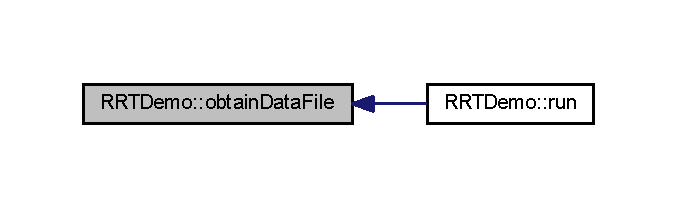
\includegraphics[width=325pt]{classRRTDemo_abe92fa34990bc750210f44a216773f42_icgraph}
\end{center}
\end{figure}


\hypertarget{classRRTDemo_aadce492558bcddbb1908233676b13c1c}{\index{R\+R\+T\+Demo@{R\+R\+T\+Demo}!scale\+View@{scale\+View}}
\index{scale\+View@{scale\+View}!R\+R\+T\+Demo@{R\+R\+T\+Demo}}
\subsubsection[{scale\+View}]{\setlength{\rightskip}{0pt plus 5cm}void R\+R\+T\+Demo\+::scale\+View (
\begin{DoxyParamCaption}
{}
\end{DoxyParamCaption}
)\hspace{0.3cm}{\ttfamily [private]}}}\label{classRRTDemo_aadce492558bcddbb1908233676b13c1c}


Stretches the \hyperlink{classLevelViewer}{Level\+Viewer} to take up the entire window and resizes the window. 



Definition at line 104 of file R\+R\+T\+Demo.\+cpp.



Here is the caller graph for this function\+:
\nopagebreak
\begin{figure}[H]
\begin{center}
\leavevmode
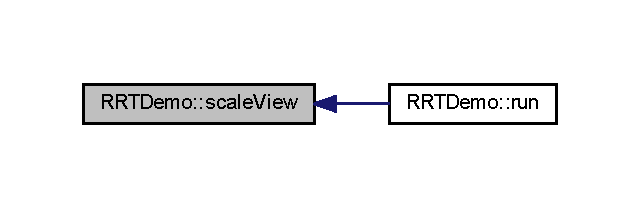
\includegraphics[width=307pt]{classRRTDemo_aadce492558bcddbb1908233676b13c1c_icgraph}
\end{center}
\end{figure}


\hypertarget{classRRTDemo_a925d73a53ebf4e1299adecffcf89b953}{\index{R\+R\+T\+Demo@{R\+R\+T\+Demo}!game\+Loop@{game\+Loop}}
\index{game\+Loop@{game\+Loop}!R\+R\+T\+Demo@{R\+R\+T\+Demo}}
\subsubsection[{game\+Loop}]{\setlength{\rightskip}{0pt plus 5cm}void R\+R\+T\+Demo\+::game\+Loop (
\begin{DoxyParamCaption}
{}
\end{DoxyParamCaption}
)\hspace{0.3cm}{\ttfamily [private]}}}\label{classRRTDemo_a925d73a53ebf4e1299adecffcf89b953}


Enters a basic game loop. 



Definition at line 135 of file R\+R\+T\+Demo.\+cpp.



Here is the caller graph for this function\+:
\nopagebreak
\begin{figure}[H]
\begin{center}
\leavevmode
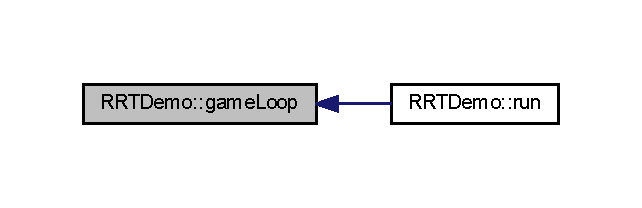
\includegraphics[width=308pt]{classRRTDemo_a925d73a53ebf4e1299adecffcf89b953_icgraph}
\end{center}
\end{figure}


\hypertarget{classRRTDemo_ad3b850c9dd02b38f8d5a8d418010a4d2}{\index{R\+R\+T\+Demo@{R\+R\+T\+Demo}!poll\+Events@{poll\+Events}}
\index{poll\+Events@{poll\+Events}!R\+R\+T\+Demo@{R\+R\+T\+Demo}}
\subsubsection[{poll\+Events}]{\setlength{\rightskip}{0pt plus 5cm}bool R\+R\+T\+Demo\+::poll\+Events (
\begin{DoxyParamCaption}
{}
\end{DoxyParamCaption}
)\hspace{0.3cm}{\ttfamily [private]}}}\label{classRRTDemo_ad3b850c9dd02b38f8d5a8d418010a4d2}


Process all window events. 

\begin{DoxyReturn}{Returns}
Whether the application should exit. 
\end{DoxyReturn}


Definition at line 164 of file R\+R\+T\+Demo.\+cpp.



Here is the caller graph for this function\+:
\nopagebreak
\begin{figure}[H]
\begin{center}
\leavevmode
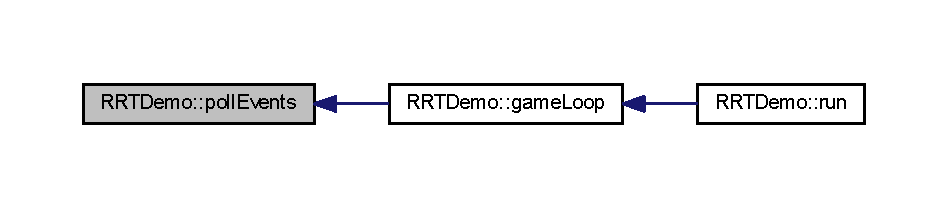
\includegraphics[width=350pt]{classRRTDemo_ad3b850c9dd02b38f8d5a8d418010a4d2_icgraph}
\end{center}
\end{figure}


\hypertarget{classRRTDemo_a5273142d4d3b5451e55d3b8609a09dca}{\index{R\+R\+T\+Demo@{R\+R\+T\+Demo}!handle\+Input@{handle\+Input}}
\index{handle\+Input@{handle\+Input}!R\+R\+T\+Demo@{R\+R\+T\+Demo}}
\subsubsection[{handle\+Input}]{\setlength{\rightskip}{0pt plus 5cm}void R\+R\+T\+Demo\+::handle\+Input (
\begin{DoxyParamCaption}
{}
\end{DoxyParamCaption}
)\hspace{0.3cm}{\ttfamily [private]}}}\label{classRRTDemo_a5273142d4d3b5451e55d3b8609a09dca}


Handles mouse input. 



Definition at line 184 of file R\+R\+T\+Demo.\+cpp.



Here is the caller graph for this function\+:
\nopagebreak
\begin{figure}[H]
\begin{center}
\leavevmode
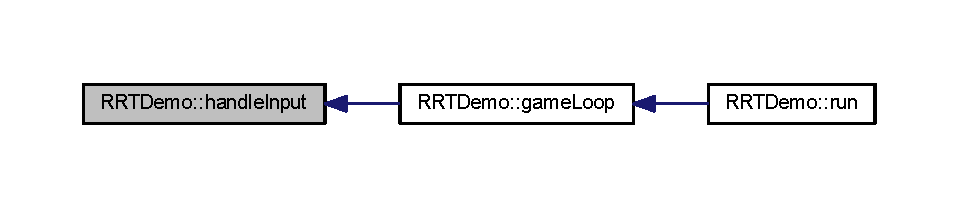
\includegraphics[width=350pt]{classRRTDemo_a5273142d4d3b5451e55d3b8609a09dca_icgraph}
\end{center}
\end{figure}




\subsection{Member Data Documentation}
\hypertarget{classRRTDemo_a74d34da51c590f616e41c1d971e2713e}{\index{R\+R\+T\+Demo@{R\+R\+T\+Demo}!m\+\_\+data@{m\+\_\+data}}
\index{m\+\_\+data@{m\+\_\+data}!R\+R\+T\+Demo@{R\+R\+T\+Demo}}
\subsubsection[{m\+\_\+data}]{\setlength{\rightskip}{0pt plus 5cm}std\+::shared\+\_\+ptr$<${\bf Level\+Data}$>$ R\+R\+T\+Demo\+::m\+\_\+data \{ nullptr \}\hspace{0.3cm}{\ttfamily [private]}}}\label{classRRTDemo_a74d34da51c590f616e41c1d971e2713e}


The level data. 



Definition at line 87 of file R\+R\+T\+Demo.\+hpp.

\hypertarget{classRRTDemo_adcef94ca094608569dbd8478b65fad08}{\index{R\+R\+T\+Demo@{R\+R\+T\+Demo}!m\+\_\+viewer@{m\+\_\+viewer}}
\index{m\+\_\+viewer@{m\+\_\+viewer}!R\+R\+T\+Demo@{R\+R\+T\+Demo}}
\subsubsection[{m\+\_\+viewer}]{\setlength{\rightskip}{0pt plus 5cm}std\+::unique\+\_\+ptr$<${\bf Level\+Viewer}$>$ R\+R\+T\+Demo\+::m\+\_\+viewer \{ nullptr \}\hspace{0.3cm}{\ttfamily [private]}}}\label{classRRTDemo_adcef94ca094608569dbd8478b65fad08}


The visual representation of the data. 



Definition at line 88 of file R\+R\+T\+Demo.\+hpp.

\hypertarget{classRRTDemo_aedde8ecc0fa074bab8c7a4d34c45c0de}{\index{R\+R\+T\+Demo@{R\+R\+T\+Demo}!m\+\_\+window@{m\+\_\+window}}
\index{m\+\_\+window@{m\+\_\+window}!R\+R\+T\+Demo@{R\+R\+T\+Demo}}
\subsubsection[{m\+\_\+window}]{\setlength{\rightskip}{0pt plus 5cm}std\+::unique\+\_\+ptr$<$sf\+::\+Render\+Window$>$ R\+R\+T\+Demo\+::m\+\_\+window \{ nullptr \}\hspace{0.3cm}{\ttfamily [private]}}}\label{classRRTDemo_aedde8ecc0fa074bab8c7a4d34c45c0de}


The window displaying the G\+U\+I of the application. 



Definition at line 89 of file R\+R\+T\+Demo.\+hpp.

\hypertarget{classRRTDemo_ae2cc9c4a77e79e09d2b0fa0dcde114c5}{\index{R\+R\+T\+Demo@{R\+R\+T\+Demo}!m\+\_\+rrt@{m\+\_\+rrt}}
\index{m\+\_\+rrt@{m\+\_\+rrt}!R\+R\+T\+Demo@{R\+R\+T\+Demo}}
\subsubsection[{m\+\_\+rrt}]{\setlength{\rightskip}{0pt plus 5cm}std\+::unique\+\_\+ptr$<${\bf R\+R\+T}$>$ R\+R\+T\+Demo\+::m\+\_\+rrt \{ \}\hspace{0.3cm}{\ttfamily [private]}}}\label{classRRTDemo_ae2cc9c4a77e79e09d2b0fa0dcde114c5}


An \hyperlink{classRRT}{R\+R\+T} object which will create a \hyperlink{classTree}{Tree} based on the \hyperlink{classLevelData}{Level\+Data}. 



Definition at line 90 of file R\+R\+T\+Demo.\+hpp.

\hypertarget{classRRTDemo_ae4c5cf25ec52db70003a96ebd0f81c62}{\index{R\+R\+T\+Demo@{R\+R\+T\+Demo}!m\+\_\+width@{m\+\_\+width}}
\index{m\+\_\+width@{m\+\_\+width}!R\+R\+T\+Demo@{R\+R\+T\+Demo}}
\subsubsection[{m\+\_\+width}]{\setlength{\rightskip}{0pt plus 5cm}const unsigned int R\+R\+T\+Demo\+::m\+\_\+width \{ 1600 \}\hspace{0.3cm}{\ttfamily [private]}}}\label{classRRTDemo_ae4c5cf25ec52db70003a96ebd0f81c62}


The maximum number of pixels wide the window can be. 



Definition at line 92 of file R\+R\+T\+Demo.\+hpp.

\hypertarget{classRRTDemo_aa9ace790edf95dc62c2b77e3ba5e567b}{\index{R\+R\+T\+Demo@{R\+R\+T\+Demo}!m\+\_\+height@{m\+\_\+height}}
\index{m\+\_\+height@{m\+\_\+height}!R\+R\+T\+Demo@{R\+R\+T\+Demo}}
\subsubsection[{m\+\_\+height}]{\setlength{\rightskip}{0pt plus 5cm}const unsigned int R\+R\+T\+Demo\+::m\+\_\+height \{ 900 \}\hspace{0.3cm}{\ttfamily [private]}}}\label{classRRTDemo_aa9ace790edf95dc62c2b77e3ba5e567b}


The maximum number of pixels tall the window can be. 



Definition at line 93 of file R\+R\+T\+Demo.\+hpp.

\hypertarget{classRRTDemo_ae776d26c1d8b700c878a572c6dcaa4c5}{\index{R\+R\+T\+Demo@{R\+R\+T\+Demo}!m\+\_\+start@{m\+\_\+start}}
\index{m\+\_\+start@{m\+\_\+start}!R\+R\+T\+Demo@{R\+R\+T\+Demo}}
\subsubsection[{m\+\_\+start}]{\setlength{\rightskip}{0pt plus 5cm}sf\+::\+Vector2i R\+R\+T\+Demo\+::m\+\_\+start \{ \}\hspace{0.3cm}{\ttfamily [private]}}}\label{classRRTDemo_ae776d26c1d8b700c878a572c6dcaa4c5}


The start point of the \hyperlink{classRRT}{R\+R\+T}. 



Definition at line 95 of file R\+R\+T\+Demo.\+hpp.

\hypertarget{classRRTDemo_a96344c80393991da942b99d30308a3da}{\index{R\+R\+T\+Demo@{R\+R\+T\+Demo}!m\+\_\+end@{m\+\_\+end}}
\index{m\+\_\+end@{m\+\_\+end}!R\+R\+T\+Demo@{R\+R\+T\+Demo}}
\subsubsection[{m\+\_\+end}]{\setlength{\rightskip}{0pt plus 5cm}sf\+::\+Vector2i R\+R\+T\+Demo\+::m\+\_\+end \{ \}\hspace{0.3cm}{\ttfamily [private]}}}\label{classRRTDemo_a96344c80393991da942b99d30308a3da}


The end point for the \hyperlink{classRRT}{R\+R\+T}. 



Definition at line 96 of file R\+R\+T\+Demo.\+hpp.



The documentation for this class was generated from the following files\+:\begin{DoxyCompactItemize}
\item 
U\+:/\+Work/\+Year2/\+G\+E\+C/\+A\+I/\+Source/\hyperlink{RRTDemo_8hpp}{R\+R\+T\+Demo.\+hpp}\item 
U\+:/\+Work/\+Year2/\+G\+E\+C/\+A\+I/\+Source/\hyperlink{RRTDemo_8cpp}{R\+R\+T\+Demo.\+cpp}\end{DoxyCompactItemize}

\hypertarget{classTree}{\section{Tree$<$ T $>$ Class Template Reference}
\label{classTree}\index{Tree$<$ T $>$@{Tree$<$ T $>$}}
}


A tree data structure containing a parent and an unlimited number of children.  




{\ttfamily \#include $<$Tree.\+hpp$>$}

\subsection*{Public Types}
\begin{DoxyCompactItemize}
\item 
using \hyperlink{classTree_a90c6da3cbc82d2a2652e7ceb19ef8f6a}{Parent} = \hyperlink{classTree}{Tree}$<$ T $>$ $\ast$
\begin{DoxyCompactList}\small\item\em The parent of the current Tree/\+Branch object. \end{DoxyCompactList}\item 
using \hyperlink{classTree_a9acb980cd198358d57fb2a6e5d65c85b}{Branch} = \hyperlink{classTree}{Tree}$<$ T $>$ $\ast$
\begin{DoxyCompactList}\small\item\em A child branch of a \hyperlink{classTree}{Tree} object. \end{DoxyCompactList}\item 
using \hyperlink{classTree_abb3de7e9104700b780c956a6da8a3582}{Branches} = std\+::vector$<$ \hyperlink{classTree_a9acb980cd198358d57fb2a6e5d65c85b}{Branch} $>$
\begin{DoxyCompactList}\small\item\em A collection of Branch objects which branch off from the \hyperlink{classTree}{Tree} object. \end{DoxyCompactList}\end{DoxyCompactItemize}
\subsection*{Public Member Functions}
\begin{DoxyCompactItemize}
\item 
\hyperlink{classTree_a3b1e8570193f05b2123b60037d039886}{Tree} (const unsigned int reserve=0\+U)
\begin{DoxyCompactList}\small\item\em Construct a tree with a reserved branch capacity. \end{DoxyCompactList}\item 
\hyperlink{classTree_aba5a7e24739444eb55f662f68990451d}{Tree} (const \hyperlink{classTree}{Tree}$<$ T $>$ \&copy)
\begin{DoxyCompactList}\small\item\em Create a copy of a \hyperlink{classTree}{Tree}, this copies in the same sense that a vector copies all dynamic memory. This cannot copy the parent node so the current point in the tree will become a root. \end{DoxyCompactList}\item 
\hyperlink{classTree}{Tree} \& \hyperlink{classTree_a44923f2569c8bcd29c08c01c35f34c5f}{operator=} (const \hyperlink{classTree}{Tree}$<$ T $>$ \&copy)
\item 
\hyperlink{classTree_a6715b29a85b15e99666b856951a676cf}{Tree} (\hyperlink{classTree}{Tree}$<$ T $>$ \&\&move)
\item 
\hyperlink{classTree}{Tree} \& \hyperlink{classTree_a6cce6e9bba6a78a237be483ff011eab3}{operator=} (\hyperlink{classTree}{Tree}$<$ T $>$ \&\&move)
\item 
\hyperlink{classTree_a04affc46d89a0ef5d517ab685c9c346e}{$\sim$\+Tree} ()
\item 
bool \hyperlink{classTree_a5057acefe504e6a599a0547f54b9fff9}{is\+Root} () const 
\begin{DoxyCompactList}\small\item\em Checks if the \hyperlink{classTree}{Tree} is a root node. \end{DoxyCompactList}\item 
bool \hyperlink{classTree_ab01ce8c8f54a3a9d954db36edecd6d9c}{is\+Tip} () const 
\begin{DoxyCompactList}\small\item\em Checks if the \hyperlink{classTree}{Tree} has any children. \end{DoxyCompactList}\item 
const T \& \hyperlink{classTree_abb747015cccad9fe63fdef2139f98973}{get\+Data} () const 
\begin{DoxyCompactList}\small\item\em Gets the data associated with this node. \end{DoxyCompactList}\item 
T \& \hyperlink{classTree_ad006a9d1e418406d911de5ed2d401827}{get\+Data} ()
\begin{DoxyCompactList}\small\item\em Gets the data associated with this node. \end{DoxyCompactList}\item 
\hyperlink{classTree_a9acb980cd198358d57fb2a6e5d65c85b}{Branch} \hyperlink{classTree_a6fea09d40751b6d724ad22350c549595}{operator\mbox{[}$\,$\mbox{]}} (const unsigned int index) const 
\begin{DoxyCompactList}\small\item\em Short hand for \hyperlink{classTree_a3f6b272bfa9033ebad14879e520bf332}{Tree\+::get\+Branch()}. \end{DoxyCompactList}\item 
unsigned int \hyperlink{classTree_a957a719014644acd75703db27ee1f36b}{get\+Branch\+Count} () const 
\begin{DoxyCompactList}\small\item\em Gets the total number of Branch objects for the \hyperlink{classTree}{Tree}. \end{DoxyCompactList}\item 
const \hyperlink{classTree_a90c6da3cbc82d2a2652e7ceb19ef8f6a}{Parent} \& \hyperlink{classTree_ad3e326b9ab23e532db1ae94d58959b41}{get\+Parent} () const 
\begin{DoxyCompactList}\small\item\em Gets the parent of the current \hyperlink{classTree}{Tree} branch. \end{DoxyCompactList}\item 
const \hyperlink{classTree_abb3de7e9104700b780c956a6da8a3582}{Branches} \& \hyperlink{classTree_a190746e8449c28314dd74bc300ea2ddf}{get\+Branches} () const 
\begin{DoxyCompactList}\small\item\em Gets the collection of Branch objects tracked by the \hyperlink{classTree}{Tree}. \end{DoxyCompactList}\item 
\hyperlink{classTree_abb3de7e9104700b780c956a6da8a3582}{Branches} \& \hyperlink{classTree_a210da94166109a9d3cc7d73497771187}{get\+Branches} ()
\begin{DoxyCompactList}\small\item\em Gets the collection of Branch objects tracked by the \hyperlink{classTree}{Tree}. \end{DoxyCompactList}\item 
\hyperlink{classTree_a9acb980cd198358d57fb2a6e5d65c85b}{Branch} \hyperlink{classTree_a3f6b272bfa9033ebad14879e520bf332}{get\+Branch} (const unsigned int index) const 
\begin{DoxyCompactList}\small\item\em Gets the branch at the current index. \end{DoxyCompactList}\item 
void \hyperlink{classTree_a47964b5ec65514701fbfed08815cece6}{set\+Data} (const T \&data)
\begin{DoxyCompactList}\small\item\em Sets the data associated with this node. \end{DoxyCompactList}\item 
void \hyperlink{classTree_a6491ed9ecd60487ccddcd20b3af9a1da}{set\+Data} (T \&\&move)
\begin{DoxyCompactList}\small\item\em Sets the data associated with this node using move semantics. \end{DoxyCompactList}\item 
void \hyperlink{classTree_a43b5e9145fa35634d0e67f048f69a01e}{set\+Branch} (const unsigned int index, const \hyperlink{classTree_a9acb980cd198358d57fb2a6e5d65c85b}{Branch} branch)
\begin{DoxyCompactList}\small\item\em Sets the Branch at the desired index. \end{DoxyCompactList}\item 
void \hyperlink{classTree_ad6d4b3f4b3584e1ef34d688b350da2ad}{clear} ()
\begin{DoxyCompactList}\small\item\em Clears the Branches object of all data. \end{DoxyCompactList}\item 
void \hyperlink{classTree_ae583fa1ebe0d58b4a94bc351add90dff}{add\+Branch} (const \hyperlink{classTree_a9acb980cd198358d57fb2a6e5d65c85b}{Branch} branch)
\begin{DoxyCompactList}\small\item\em Adds a Branch to the end of the collection of Branch objects. \end{DoxyCompactList}\item 
void \hyperlink{classTree_a8515bc0f3003f1d13cbe582cedfbe6ae}{add\+Branch} (const unsigned int index, const \hyperlink{classTree_a9acb980cd198358d57fb2a6e5d65c85b}{Branch} branch)
\begin{DoxyCompactList}\small\item\em Adds a Branch at the specified index, this can be very slow. \end{DoxyCompactList}\item 
void \hyperlink{classTree_ac851df39dc89e9a8c60b4898d8012fd7}{remove\+Branch} (const unsigned int index)
\begin{DoxyCompactList}\small\item\em Removes a Branch from the Branches object, this is fast but changes the order. \end{DoxyCompactList}\item 
void \hyperlink{classTree_a8976206e549d5e8eb127928bdfb35971}{remove\+Branch} (const \hyperlink{classTree_a9acb980cd198358d57fb2a6e5d65c85b}{Branch} branch)
\begin{DoxyCompactList}\small\item\em Removes a Branch from the Branches object, this is fast but changes the order. \end{DoxyCompactList}\item 
void \hyperlink{classTree_a05cffee2182f101a56aec75bd4229f52}{remove\+Branch\+Ordered} (const unsigned int index)
\begin{DoxyCompactList}\small\item\em Removes a Branch from the Branches object whilst maintaining the order. \end{DoxyCompactList}\item 
void \hyperlink{classTree_a43deacc7a03b8a86c0239de1ebbbd2c5}{remove\+Branch\+Ordered} (const \hyperlink{classTree_a9acb980cd198358d57fb2a6e5d65c85b}{Branch} branch)
\begin{DoxyCompactList}\small\item\em Removes a Branch from the Branches object whilst maintaining the order. \end{DoxyCompactList}\item 
unsigned int \hyperlink{classTree_aa680ed5fc071515455a20a13592e3900}{find\+Index} (const \hyperlink{classTree_a9acb980cd198358d57fb2a6e5d65c85b}{Branch} branch) const 
\begin{DoxyCompactList}\small\item\em Finds the index of the given branch. \end{DoxyCompactList}\end{DoxyCompactItemize}
\subsection*{Private Attributes}
\begin{DoxyCompactItemize}
\item 
T \hyperlink{classTree_a4ace53b9a58c7c6a96b85be871471f62}{m\+\_\+data} \{ \}
\begin{DoxyCompactList}\small\item\em The data of the node. \end{DoxyCompactList}\item 
\hyperlink{classTree_a90c6da3cbc82d2a2652e7ceb19ef8f6a}{Parent} \hyperlink{classTree_ac742fce39cb2288663f891d77c3e4748}{m\+\_\+parent} \{ \}
\begin{DoxyCompactList}\small\item\em The parent of the current branch of a \hyperlink{classTree}{Tree}. \end{DoxyCompactList}\item 
\hyperlink{classTree_abb3de7e9104700b780c956a6da8a3582}{Branches} \hyperlink{classTree_ab9520d0aea2873cd23caa31f6d6aa823}{m\+\_\+branches} \{ \}
\begin{DoxyCompactList}\small\item\em The child branches of the current branch of a \hyperlink{classTree}{Tree}. \end{DoxyCompactList}\end{DoxyCompactItemize}


\subsection{Detailed Description}
\subsubsection*{template$<$typename T$>$class Tree$<$ T $>$}

A tree data structure containing a parent and an unlimited number of children. 



Definition at line 14 of file Tree.\+hpp.



\subsection{Member Typedef Documentation}
\hypertarget{classTree_a90c6da3cbc82d2a2652e7ceb19ef8f6a}{\index{Tree@{Tree}!Parent@{Parent}}
\index{Parent@{Parent}!Tree@{Tree}}
\subsubsection[{Parent}]{\setlength{\rightskip}{0pt plus 5cm}template$<$typename T$>$ using {\bf Tree}$<$ T $>$\+::{\bf Parent} =  {\bf Tree}$<$T$>$$\ast$}}\label{classTree_a90c6da3cbc82d2a2652e7ceb19ef8f6a}


The parent of the current Tree/\+Branch object. 



Definition at line 23 of file Tree.\+hpp.

\hypertarget{classTree_a9acb980cd198358d57fb2a6e5d65c85b}{\index{Tree@{Tree}!Branch@{Branch}}
\index{Branch@{Branch}!Tree@{Tree}}
\subsubsection[{Branch}]{\setlength{\rightskip}{0pt plus 5cm}template$<$typename T$>$ using {\bf Tree}$<$ T $>$\+::{\bf Branch} =  {\bf Tree}$<$T$>$$\ast$}}\label{classTree_a9acb980cd198358d57fb2a6e5d65c85b}


A child branch of a \hyperlink{classTree}{Tree} object. 



Definition at line 26 of file Tree.\+hpp.

\hypertarget{classTree_abb3de7e9104700b780c956a6da8a3582}{\index{Tree@{Tree}!Branches@{Branches}}
\index{Branches@{Branches}!Tree@{Tree}}
\subsubsection[{Branches}]{\setlength{\rightskip}{0pt plus 5cm}template$<$typename T$>$ using {\bf Tree}$<$ T $>$\+::{\bf Branches} =  std\+::vector$<${\bf Branch}$>$}}\label{classTree_abb3de7e9104700b780c956a6da8a3582}


A collection of Branch objects which branch off from the \hyperlink{classTree}{Tree} object. 



Definition at line 29 of file Tree.\+hpp.



\subsection{Constructor \& Destructor Documentation}
\hypertarget{classTree_a3b1e8570193f05b2123b60037d039886}{\index{Tree@{Tree}!Tree@{Tree}}
\index{Tree@{Tree}!Tree@{Tree}}
\subsubsection[{Tree}]{\setlength{\rightskip}{0pt plus 5cm}template$<$typename T $>$ {\bf Tree}$<$ T $>$\+::{\bf Tree} (
\begin{DoxyParamCaption}
\item[{const unsigned int}]{reserve = {\ttfamily 0U}}
\end{DoxyParamCaption}
)}}\label{classTree_a3b1e8570193f05b2123b60037d039886}


Construct a tree with a reserved branch capacity. 


\begin{DoxyParams}{Parameters}
{\em reserve} & How much capacity to reserve. \\
\hline
\end{DoxyParams}


Definition at line 162 of file Tree.\+hpp.

\hypertarget{classTree_aba5a7e24739444eb55f662f68990451d}{\index{Tree@{Tree}!Tree@{Tree}}
\index{Tree@{Tree}!Tree@{Tree}}
\subsubsection[{Tree}]{\setlength{\rightskip}{0pt plus 5cm}template$<$typename T$>$ {\bf Tree}$<$ T $>$\+::{\bf Tree} (
\begin{DoxyParamCaption}
\item[{const {\bf Tree}$<$ T $>$ \&}]{copy}
\end{DoxyParamCaption}
)}}\label{classTree_aba5a7e24739444eb55f662f68990451d}


Create a copy of a \hyperlink{classTree}{Tree}, this copies in the same sense that a vector copies all dynamic memory. This cannot copy the parent node so the current point in the tree will become a root. 



Definition at line 169 of file Tree.\+hpp.

\hypertarget{classTree_a6715b29a85b15e99666b856951a676cf}{\index{Tree@{Tree}!Tree@{Tree}}
\index{Tree@{Tree}!Tree@{Tree}}
\subsubsection[{Tree}]{\setlength{\rightskip}{0pt plus 5cm}template$<$typename T$>$ {\bf Tree}$<$ T $>$\+::{\bf Tree} (
\begin{DoxyParamCaption}
\item[{{\bf Tree}$<$ T $>$ \&\&}]{move}
\end{DoxyParamCaption}
)}}\label{classTree_a6715b29a85b15e99666b856951a676cf}


Definition at line 176 of file Tree.\+hpp.

\hypertarget{classTree_a04affc46d89a0ef5d517ab685c9c346e}{\index{Tree@{Tree}!````~Tree@{$\sim$\+Tree}}
\index{````~Tree@{$\sim$\+Tree}!Tree@{Tree}}
\subsubsection[{$\sim$\+Tree}]{\setlength{\rightskip}{0pt plus 5cm}template$<$typename T $>$ {\bf Tree}$<$ T $>$\+::$\sim${\bf Tree} (
\begin{DoxyParamCaption}
{}
\end{DoxyParamCaption}
)}}\label{classTree_a04affc46d89a0ef5d517ab685c9c346e}


Definition at line 211 of file Tree.\+hpp.



\subsection{Member Function Documentation}
\hypertarget{classTree_a44923f2569c8bcd29c08c01c35f34c5f}{\index{Tree@{Tree}!operator=@{operator=}}
\index{operator=@{operator=}!Tree@{Tree}}
\subsubsection[{operator=}]{\setlength{\rightskip}{0pt plus 5cm}template$<$typename T$>$ {\bf Tree}$<$ T $>$ \& {\bf Tree}$<$ T $>$\+::operator= (
\begin{DoxyParamCaption}
\item[{const {\bf Tree}$<$ T $>$ \&}]{copy}
\end{DoxyParamCaption}
)}}\label{classTree_a44923f2569c8bcd29c08c01c35f34c5f}


Definition at line 183 of file Tree.\+hpp.

\hypertarget{classTree_a6cce6e9bba6a78a237be483ff011eab3}{\index{Tree@{Tree}!operator=@{operator=}}
\index{operator=@{operator=}!Tree@{Tree}}
\subsubsection[{operator=}]{\setlength{\rightskip}{0pt plus 5cm}template$<$typename T$>$ {\bf Tree}$<$ T $>$ \& {\bf Tree}$<$ T $>$\+::operator= (
\begin{DoxyParamCaption}
\item[{{\bf Tree}$<$ T $>$ \&\&}]{move}
\end{DoxyParamCaption}
)}}\label{classTree_a6cce6e9bba6a78a237be483ff011eab3}


Definition at line 195 of file Tree.\+hpp.

\hypertarget{classTree_a5057acefe504e6a599a0547f54b9fff9}{\index{Tree@{Tree}!is\+Root@{is\+Root}}
\index{is\+Root@{is\+Root}!Tree@{Tree}}
\subsubsection[{is\+Root}]{\setlength{\rightskip}{0pt plus 5cm}template$<$typename T$>$ bool {\bf Tree}$<$ T $>$\+::is\+Root (
\begin{DoxyParamCaption}
{}
\end{DoxyParamCaption}
) const\hspace{0.3cm}{\ttfamily [inline]}}}\label{classTree_a5057acefe504e6a599a0547f54b9fff9}


Checks if the \hyperlink{classTree}{Tree} is a root node. 



Definition at line 57 of file Tree.\+hpp.

\hypertarget{classTree_ab01ce8c8f54a3a9d954db36edecd6d9c}{\index{Tree@{Tree}!is\+Tip@{is\+Tip}}
\index{is\+Tip@{is\+Tip}!Tree@{Tree}}
\subsubsection[{is\+Tip}]{\setlength{\rightskip}{0pt plus 5cm}template$<$typename T$>$ bool {\bf Tree}$<$ T $>$\+::is\+Tip (
\begin{DoxyParamCaption}
{}
\end{DoxyParamCaption}
) const\hspace{0.3cm}{\ttfamily [inline]}}}\label{classTree_ab01ce8c8f54a3a9d954db36edecd6d9c}


Checks if the \hyperlink{classTree}{Tree} has any children. 



Definition at line 60 of file Tree.\+hpp.

\hypertarget{classTree_abb747015cccad9fe63fdef2139f98973}{\index{Tree@{Tree}!get\+Data@{get\+Data}}
\index{get\+Data@{get\+Data}!Tree@{Tree}}
\subsubsection[{get\+Data}]{\setlength{\rightskip}{0pt plus 5cm}template$<$typename T$>$ const T\& {\bf Tree}$<$ T $>$\+::get\+Data (
\begin{DoxyParamCaption}
{}
\end{DoxyParamCaption}
) const\hspace{0.3cm}{\ttfamily [inline]}}}\label{classTree_abb747015cccad9fe63fdef2139f98973}


Gets the data associated with this node. 

\begin{DoxyReturn}{Returns}
A read-\/only reference to the data. 
\end{DoxyReturn}


Definition at line 64 of file Tree.\+hpp.

\hypertarget{classTree_ad006a9d1e418406d911de5ed2d401827}{\index{Tree@{Tree}!get\+Data@{get\+Data}}
\index{get\+Data@{get\+Data}!Tree@{Tree}}
\subsubsection[{get\+Data}]{\setlength{\rightskip}{0pt plus 5cm}template$<$typename T$>$ T\& {\bf Tree}$<$ T $>$\+::get\+Data (
\begin{DoxyParamCaption}
{}
\end{DoxyParamCaption}
)\hspace{0.3cm}{\ttfamily [inline]}}}\label{classTree_ad006a9d1e418406d911de5ed2d401827}


Gets the data associated with this node. 

\begin{DoxyReturn}{Returns}
A modifiable reference to the data. 
\end{DoxyReturn}


Definition at line 68 of file Tree.\+hpp.

\hypertarget{classTree_a6fea09d40751b6d724ad22350c549595}{\index{Tree@{Tree}!operator\mbox{[}$\,$\mbox{]}@{operator[]}}
\index{operator\mbox{[}$\,$\mbox{]}@{operator[]}!Tree@{Tree}}
\subsubsection[{operator[]}]{\setlength{\rightskip}{0pt plus 5cm}template$<$typename T$>$ {\bf Branch} {\bf Tree}$<$ T $>$\+::operator\mbox{[}$\,$\mbox{]} (
\begin{DoxyParamCaption}
\item[{const unsigned int}]{index}
\end{DoxyParamCaption}
) const\hspace{0.3cm}{\ttfamily [inline]}}}\label{classTree_a6fea09d40751b6d724ad22350c549595}


Short hand for \hyperlink{classTree_a3f6b272bfa9033ebad14879e520bf332}{Tree\+::get\+Branch()}. 



Definition at line 71 of file Tree.\+hpp.

\hypertarget{classTree_a957a719014644acd75703db27ee1f36b}{\index{Tree@{Tree}!get\+Branch\+Count@{get\+Branch\+Count}}
\index{get\+Branch\+Count@{get\+Branch\+Count}!Tree@{Tree}}
\subsubsection[{get\+Branch\+Count}]{\setlength{\rightskip}{0pt plus 5cm}template$<$typename T$>$ unsigned int {\bf Tree}$<$ T $>$\+::get\+Branch\+Count (
\begin{DoxyParamCaption}
{}
\end{DoxyParamCaption}
) const\hspace{0.3cm}{\ttfamily [inline]}}}\label{classTree_a957a719014644acd75703db27ee1f36b}


Gets the total number of Branch objects for the \hyperlink{classTree}{Tree}. 



Definition at line 74 of file Tree.\+hpp.

\hypertarget{classTree_ad3e326b9ab23e532db1ae94d58959b41}{\index{Tree@{Tree}!get\+Parent@{get\+Parent}}
\index{get\+Parent@{get\+Parent}!Tree@{Tree}}
\subsubsection[{get\+Parent}]{\setlength{\rightskip}{0pt plus 5cm}template$<$typename T$>$ const {\bf Parent}\& {\bf Tree}$<$ T $>$\+::get\+Parent (
\begin{DoxyParamCaption}
{}
\end{DoxyParamCaption}
) const\hspace{0.3cm}{\ttfamily [inline]}}}\label{classTree_ad3e326b9ab23e532db1ae94d58959b41}


Gets the parent of the current \hyperlink{classTree}{Tree} branch. 



Definition at line 77 of file Tree.\+hpp.

\hypertarget{classTree_a190746e8449c28314dd74bc300ea2ddf}{\index{Tree@{Tree}!get\+Branches@{get\+Branches}}
\index{get\+Branches@{get\+Branches}!Tree@{Tree}}
\subsubsection[{get\+Branches}]{\setlength{\rightskip}{0pt plus 5cm}template$<$typename T$>$ const {\bf Branches}\& {\bf Tree}$<$ T $>$\+::get\+Branches (
\begin{DoxyParamCaption}
{}
\end{DoxyParamCaption}
) const\hspace{0.3cm}{\ttfamily [inline]}}}\label{classTree_a190746e8449c28314dd74bc300ea2ddf}


Gets the collection of Branch objects tracked by the \hyperlink{classTree}{Tree}. 

\begin{DoxyReturn}{Returns}
A read-\/only reference. 
\end{DoxyReturn}


Definition at line 81 of file Tree.\+hpp.

\hypertarget{classTree_a210da94166109a9d3cc7d73497771187}{\index{Tree@{Tree}!get\+Branches@{get\+Branches}}
\index{get\+Branches@{get\+Branches}!Tree@{Tree}}
\subsubsection[{get\+Branches}]{\setlength{\rightskip}{0pt plus 5cm}template$<$typename T$>$ {\bf Branches}\& {\bf Tree}$<$ T $>$\+::get\+Branches (
\begin{DoxyParamCaption}
{}
\end{DoxyParamCaption}
)\hspace{0.3cm}{\ttfamily [inline]}}}\label{classTree_a210da94166109a9d3cc7d73497771187}


Gets the collection of Branch objects tracked by the \hyperlink{classTree}{Tree}. 

\begin{DoxyReturn}{Returns}
A modifiable reference. 
\end{DoxyReturn}


Definition at line 85 of file Tree.\+hpp.

\hypertarget{classTree_a3f6b272bfa9033ebad14879e520bf332}{\index{Tree@{Tree}!get\+Branch@{get\+Branch}}
\index{get\+Branch@{get\+Branch}!Tree@{Tree}}
\subsubsection[{get\+Branch}]{\setlength{\rightskip}{0pt plus 5cm}template$<$typename T $>$ {\bf Tree}$<$ T $>$\+::{\bf Branch} {\bf Tree}$<$ T $>$\+::get\+Branch (
\begin{DoxyParamCaption}
\item[{const unsigned int}]{index}
\end{DoxyParamCaption}
) const}}\label{classTree_a3f6b272bfa9033ebad14879e520bf332}


Gets the branch at the current index. 



Definition at line 230 of file Tree.\+hpp.



Here is the caller graph for this function\+:
\nopagebreak
\begin{figure}[H]
\begin{center}
\leavevmode
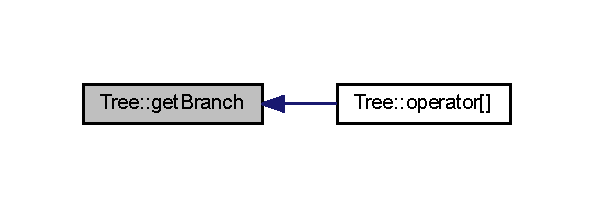
\includegraphics[width=285pt]{classTree_a3f6b272bfa9033ebad14879e520bf332_icgraph}
\end{center}
\end{figure}


\hypertarget{classTree_a47964b5ec65514701fbfed08815cece6}{\index{Tree@{Tree}!set\+Data@{set\+Data}}
\index{set\+Data@{set\+Data}!Tree@{Tree}}
\subsubsection[{set\+Data}]{\setlength{\rightskip}{0pt plus 5cm}template$<$typename T$>$ void {\bf Tree}$<$ T $>$\+::set\+Data (
\begin{DoxyParamCaption}
\item[{const T \&}]{data}
\end{DoxyParamCaption}
)\hspace{0.3cm}{\ttfamily [inline]}}}\label{classTree_a47964b5ec65514701fbfed08815cece6}


Sets the data associated with this node. 



Definition at line 91 of file Tree.\+hpp.

\hypertarget{classTree_a6491ed9ecd60487ccddcd20b3af9a1da}{\index{Tree@{Tree}!set\+Data@{set\+Data}}
\index{set\+Data@{set\+Data}!Tree@{Tree}}
\subsubsection[{set\+Data}]{\setlength{\rightskip}{0pt plus 5cm}template$<$typename T$>$ void {\bf Tree}$<$ T $>$\+::set\+Data (
\begin{DoxyParamCaption}
\item[{T \&\&}]{move}
\end{DoxyParamCaption}
)\hspace{0.3cm}{\ttfamily [inline]}}}\label{classTree_a6491ed9ecd60487ccddcd20b3af9a1da}


Sets the data associated with this node using move semantics. 



Definition at line 94 of file Tree.\+hpp.

\hypertarget{classTree_a43b5e9145fa35634d0e67f048f69a01e}{\index{Tree@{Tree}!set\+Branch@{set\+Branch}}
\index{set\+Branch@{set\+Branch}!Tree@{Tree}}
\subsubsection[{set\+Branch}]{\setlength{\rightskip}{0pt plus 5cm}template$<$typename T $>$ void {\bf Tree}$<$ T $>$\+::set\+Branch (
\begin{DoxyParamCaption}
\item[{const unsigned int}]{index, }
\item[{const {\bf Branch}}]{branch}
\end{DoxyParamCaption}
)}}\label{classTree_a43b5e9145fa35634d0e67f048f69a01e}


Sets the Branch at the desired index. 


\begin{DoxyParams}{Parameters}
{\em index} & The index to set the Branch to. \\
\hline
{\em branch} & The branch to use. \\
\hline
\end{DoxyParams}


Definition at line 240 of file Tree.\+hpp.

\hypertarget{classTree_ad6d4b3f4b3584e1ef34d688b350da2ad}{\index{Tree@{Tree}!clear@{clear}}
\index{clear@{clear}!Tree@{Tree}}
\subsubsection[{clear}]{\setlength{\rightskip}{0pt plus 5cm}template$<$typename T$>$ void {\bf Tree}$<$ T $>$\+::clear (
\begin{DoxyParamCaption}
{}
\end{DoxyParamCaption}
)\hspace{0.3cm}{\ttfamily [inline]}}}\label{classTree_ad6d4b3f4b3584e1ef34d688b350da2ad}


Clears the Branches object of all data. 



Definition at line 107 of file Tree.\+hpp.

\hypertarget{classTree_ae583fa1ebe0d58b4a94bc351add90dff}{\index{Tree@{Tree}!add\+Branch@{add\+Branch}}
\index{add\+Branch@{add\+Branch}!Tree@{Tree}}
\subsubsection[{add\+Branch}]{\setlength{\rightskip}{0pt plus 5cm}template$<$typename T $>$ void {\bf Tree}$<$ T $>$\+::add\+Branch (
\begin{DoxyParamCaption}
\item[{const {\bf Branch}}]{branch}
\end{DoxyParamCaption}
)}}\label{classTree_ae583fa1ebe0d58b4a94bc351add90dff}


Adds a Branch to the end of the collection of Branch objects. 


\begin{DoxyParams}{Parameters}
{\em branch} & The Branch object to add. \\
\hline
\end{DoxyParams}


Definition at line 254 of file Tree.\+hpp.

\hypertarget{classTree_a8515bc0f3003f1d13cbe582cedfbe6ae}{\index{Tree@{Tree}!add\+Branch@{add\+Branch}}
\index{add\+Branch@{add\+Branch}!Tree@{Tree}}
\subsubsection[{add\+Branch}]{\setlength{\rightskip}{0pt plus 5cm}template$<$typename T $>$ void {\bf Tree}$<$ T $>$\+::add\+Branch (
\begin{DoxyParamCaption}
\item[{const unsigned int}]{index, }
\item[{const {\bf Branch}}]{branch}
\end{DoxyParamCaption}
)}}\label{classTree_a8515bc0f3003f1d13cbe582cedfbe6ae}


Adds a Branch at the specified index, this can be very slow. 


\begin{DoxyParams}{Parameters}
{\em index} & The index to add the branch at. \\
\hline
{\em branch} & The branch to add. \\
\hline
\end{DoxyParams}


Definition at line 261 of file Tree.\+hpp.

\hypertarget{classTree_ac851df39dc89e9a8c60b4898d8012fd7}{\index{Tree@{Tree}!remove\+Branch@{remove\+Branch}}
\index{remove\+Branch@{remove\+Branch}!Tree@{Tree}}
\subsubsection[{remove\+Branch}]{\setlength{\rightskip}{0pt plus 5cm}template$<$typename T $>$ void {\bf Tree}$<$ T $>$\+::remove\+Branch (
\begin{DoxyParamCaption}
\item[{const unsigned int}]{index}
\end{DoxyParamCaption}
)}}\label{classTree_ac851df39dc89e9a8c60b4898d8012fd7}


Removes a Branch from the Branches object, this is fast but changes the order. 


\begin{DoxyParams}{Parameters}
{\em index} & The index of the Branch to remove. \\
\hline
\end{DoxyParams}


Definition at line 272 of file Tree.\+hpp.

\hypertarget{classTree_a8976206e549d5e8eb127928bdfb35971}{\index{Tree@{Tree}!remove\+Branch@{remove\+Branch}}
\index{remove\+Branch@{remove\+Branch}!Tree@{Tree}}
\subsubsection[{remove\+Branch}]{\setlength{\rightskip}{0pt plus 5cm}template$<$typename T $>$ void {\bf Tree}$<$ T $>$\+::remove\+Branch (
\begin{DoxyParamCaption}
\item[{const {\bf Branch}}]{branch}
\end{DoxyParamCaption}
)}}\label{classTree_a8976206e549d5e8eb127928bdfb35971}


Removes a Branch from the Branches object, this is fast but changes the order. 


\begin{DoxyParams}{Parameters}
{\em branch} & The Branch to remove. \\
\hline
\end{DoxyParams}


Definition at line 286 of file Tree.\+hpp.

\hypertarget{classTree_a05cffee2182f101a56aec75bd4229f52}{\index{Tree@{Tree}!remove\+Branch\+Ordered@{remove\+Branch\+Ordered}}
\index{remove\+Branch\+Ordered@{remove\+Branch\+Ordered}!Tree@{Tree}}
\subsubsection[{remove\+Branch\+Ordered}]{\setlength{\rightskip}{0pt plus 5cm}template$<$typename T $>$ void {\bf Tree}$<$ T $>$\+::remove\+Branch\+Ordered (
\begin{DoxyParamCaption}
\item[{const unsigned int}]{index}
\end{DoxyParamCaption}
)}}\label{classTree_a05cffee2182f101a56aec75bd4229f52}


Removes a Branch from the Branches object whilst maintaining the order. 


\begin{DoxyParams}{Parameters}
{\em index} & The index of the Branch to remove. \\
\hline
\end{DoxyParams}


Definition at line 293 of file Tree.\+hpp.

\hypertarget{classTree_a43deacc7a03b8a86c0239de1ebbbd2c5}{\index{Tree@{Tree}!remove\+Branch\+Ordered@{remove\+Branch\+Ordered}}
\index{remove\+Branch\+Ordered@{remove\+Branch\+Ordered}!Tree@{Tree}}
\subsubsection[{remove\+Branch\+Ordered}]{\setlength{\rightskip}{0pt plus 5cm}template$<$typename T $>$ void {\bf Tree}$<$ T $>$\+::remove\+Branch\+Ordered (
\begin{DoxyParamCaption}
\item[{const {\bf Branch}}]{branch}
\end{DoxyParamCaption}
)}}\label{classTree_a43deacc7a03b8a86c0239de1ebbbd2c5}


Removes a Branch from the Branches object whilst maintaining the order. 


\begin{DoxyParams}{Parameters}
{\em branch} & The Branch to remove. \\
\hline
\end{DoxyParams}


Definition at line 304 of file Tree.\+hpp.

\hypertarget{classTree_aa680ed5fc071515455a20a13592e3900}{\index{Tree@{Tree}!find\+Index@{find\+Index}}
\index{find\+Index@{find\+Index}!Tree@{Tree}}
\subsubsection[{find\+Index}]{\setlength{\rightskip}{0pt plus 5cm}template$<$typename T $>$ unsigned int {\bf Tree}$<$ T $>$\+::find\+Index (
\begin{DoxyParamCaption}
\item[{const {\bf Branch}}]{branch}
\end{DoxyParamCaption}
) const}}\label{classTree_aa680ed5fc071515455a20a13592e3900}


Finds the index of the given branch. 


\begin{DoxyParams}{Parameters}
{\em branch} & The branch to look for. \\
\hline
\end{DoxyParams}
\begin{DoxyReturn}{Returns}
The index, \hyperlink{classTree_a957a719014644acd75703db27ee1f36b}{Tree\+::get\+Branch\+Count()} if it does not exist. 
\end{DoxyReturn}


Definition at line 315 of file Tree.\+hpp.



\subsection{Member Data Documentation}
\hypertarget{classTree_a4ace53b9a58c7c6a96b85be871471f62}{\index{Tree@{Tree}!m\+\_\+data@{m\+\_\+data}}
\index{m\+\_\+data@{m\+\_\+data}!Tree@{Tree}}
\subsubsection[{m\+\_\+data}]{\setlength{\rightskip}{0pt plus 5cm}template$<$typename T$>$ T {\bf Tree}$<$ T $>$\+::m\+\_\+data \{ \}\hspace{0.3cm}{\ttfamily [private]}}}\label{classTree_a4ace53b9a58c7c6a96b85be871471f62}


The data of the node. 



Definition at line 151 of file Tree.\+hpp.

\hypertarget{classTree_ac742fce39cb2288663f891d77c3e4748}{\index{Tree@{Tree}!m\+\_\+parent@{m\+\_\+parent}}
\index{m\+\_\+parent@{m\+\_\+parent}!Tree@{Tree}}
\subsubsection[{m\+\_\+parent}]{\setlength{\rightskip}{0pt plus 5cm}template$<$typename T$>$ {\bf Parent} {\bf Tree}$<$ T $>$\+::m\+\_\+parent \{ \}\hspace{0.3cm}{\ttfamily [private]}}}\label{classTree_ac742fce39cb2288663f891d77c3e4748}


The parent of the current branch of a \hyperlink{classTree}{Tree}. 



Definition at line 152 of file Tree.\+hpp.

\hypertarget{classTree_ab9520d0aea2873cd23caa31f6d6aa823}{\index{Tree@{Tree}!m\+\_\+branches@{m\+\_\+branches}}
\index{m\+\_\+branches@{m\+\_\+branches}!Tree@{Tree}}
\subsubsection[{m\+\_\+branches}]{\setlength{\rightskip}{0pt plus 5cm}template$<$typename T$>$ {\bf Branches} {\bf Tree}$<$ T $>$\+::m\+\_\+branches \{ \}\hspace{0.3cm}{\ttfamily [private]}}}\label{classTree_ab9520d0aea2873cd23caa31f6d6aa823}


The child branches of the current branch of a \hyperlink{classTree}{Tree}. 



Definition at line 153 of file Tree.\+hpp.



The documentation for this class was generated from the following file\+:\begin{DoxyCompactItemize}
\item 
U\+:/\+Work/\+Year2/\+G\+E\+C/\+A\+I/\+Source/\+R\+R\+T/\hyperlink{Tree_8hpp}{Tree.\+hpp}\end{DoxyCompactItemize}

\chapter{File Documentation}
\hypertarget{LevelData_8cpp}{\section{U\+:/\+Work/\+Year2/\+G\+E\+C/\+A\+I/\+Source/\+Level/\+Level\+Data.cpp File Reference}
\label{LevelData_8cpp}\index{U\+:/\+Work/\+Year2/\+G\+E\+C/\+A\+I/\+Source/\+Level/\+Level\+Data.\+cpp@{U\+:/\+Work/\+Year2/\+G\+E\+C/\+A\+I/\+Source/\+Level/\+Level\+Data.\+cpp}}
}
{\ttfamily \#include \char`\"{}Level\+Data.\+hpp\char`\"{}}\\*
{\ttfamily \#include $<$cassert$>$}\\*
{\ttfamily \#include $<$fstream$>$}\\*
{\ttfamily \#include $<$stdexcept$>$}\\*
{\ttfamily \#include $<$utility$>$}\\*
Include dependency graph for Level\+Data.\+cpp\+:
\nopagebreak
\begin{figure}[H]
\begin{center}
\leavevmode
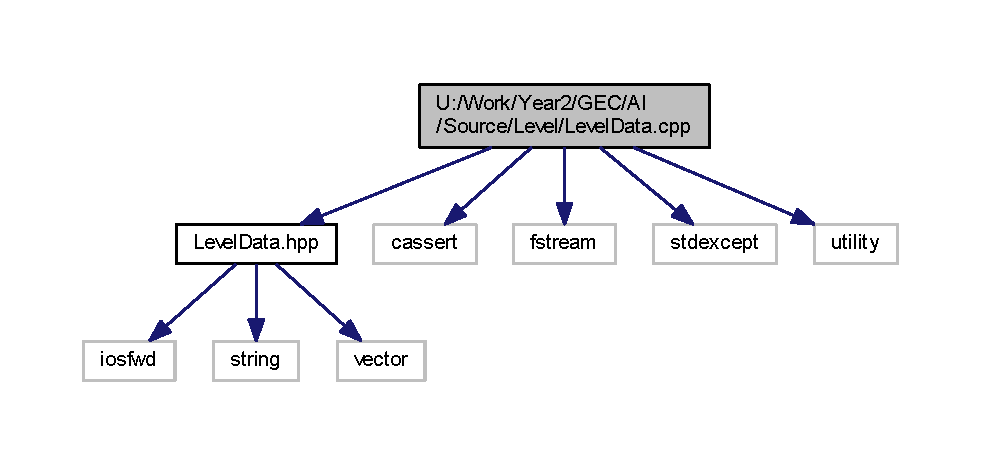
\includegraphics[width=350pt]{LevelData_8cpp__incl}
\end{center}
\end{figure}

\hypertarget{LevelData_8hpp}{\section{U\+:/\+Work/\+Year2/\+G\+E\+C/\+A\+I/\+Source/\+Level/\+Level\+Data.hpp File Reference}
\label{LevelData_8hpp}\index{U\+:/\+Work/\+Year2/\+G\+E\+C/\+A\+I/\+Source/\+Level/\+Level\+Data.\+hpp@{U\+:/\+Work/\+Year2/\+G\+E\+C/\+A\+I/\+Source/\+Level/\+Level\+Data.\+hpp}}
}
{\ttfamily \#include $<$iosfwd$>$}\\*
{\ttfamily \#include $<$string$>$}\\*
{\ttfamily \#include $<$vector$>$}\\*
Include dependency graph for Level\+Data.\+hpp\+:
\nopagebreak
\begin{figure}[H]
\begin{center}
\leavevmode
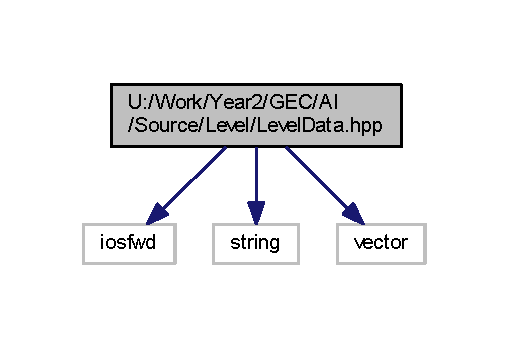
\includegraphics[width=244pt]{LevelData_8hpp__incl}
\end{center}
\end{figure}
This graph shows which files directly or indirectly include this file\+:
\nopagebreak
\begin{figure}[H]
\begin{center}
\leavevmode
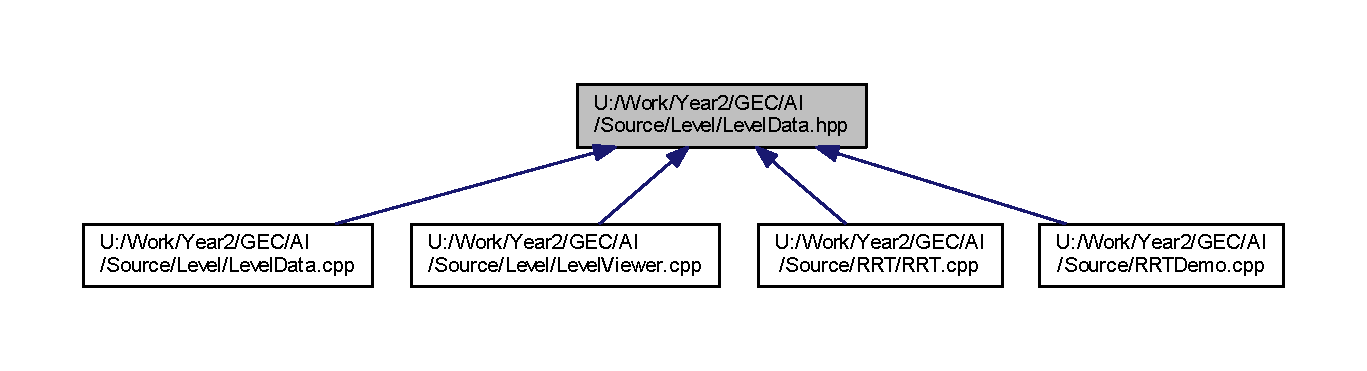
\includegraphics[width=350pt]{LevelData_8hpp__dep__incl}
\end{center}
\end{figure}
\subsection*{Classes}
\begin{DoxyCompactItemize}
\item 
class \hyperlink{classLevelData}{Level\+Data}
\begin{DoxyCompactList}\small\item\em Represents a loaded level, this contains the dimensions and tiles of a level which can be used for A\+I algorithms. \end{DoxyCompactList}\end{DoxyCompactItemize}
\subsection*{Enumerations}
\begin{DoxyCompactItemize}
\item 
enum \hyperlink{LevelData_8hpp_a47dee72188473c57343127b1a5843398}{Tile\+Type} \+: char \{ \\*
\hyperlink{LevelData_8hpp_a47dee72188473c57343127b1a5843398a4ccfea7a25fae3c1d31555f0856d2b42}{Tile\+Type\+::\+Terrain}, 
\hyperlink{LevelData_8hpp_a47dee72188473c57343127b1a5843398a46dc1018ac1d8fca7c2752a61ce2fd0f}{Tile\+Type\+::\+Out\+Of\+Bounds}, 
\hyperlink{LevelData_8hpp_a47dee72188473c57343127b1a5843398a3b0c14770e6bd663518496da60f524da}{Tile\+Type\+::\+Tree}, 
\hyperlink{LevelData_8hpp_a47dee72188473c57343127b1a5843398a2b6f48ac3e1c531576cb06c03d0cb81b}{Tile\+Type\+::\+Swamp}, 
\\*
\hyperlink{LevelData_8hpp_a47dee72188473c57343127b1a5843398a27634ff8002b12e75d98e07ccd005d18}{Tile\+Type\+::\+Water}
 \}
\begin{DoxyCompactList}\small\item\em An enum containing a representation of each tile type. \end{DoxyCompactList}\end{DoxyCompactItemize}


\subsection{Enumeration Type Documentation}
\hypertarget{LevelData_8hpp_a47dee72188473c57343127b1a5843398}{\index{Level\+Data.\+hpp@{Level\+Data.\+hpp}!Tile\+Type@{Tile\+Type}}
\index{Tile\+Type@{Tile\+Type}!Level\+Data.\+hpp@{Level\+Data.\+hpp}}
\subsubsection[{Tile\+Type}]{\setlength{\rightskip}{0pt plus 5cm}enum {\bf Tile\+Type} \+: char\hspace{0.3cm}{\ttfamily [strong]}}}\label{LevelData_8hpp_a47dee72188473c57343127b1a5843398}


An enum containing a representation of each tile type. 

\begin{Desc}
\item[Enumerator]\par
\begin{description}
\index{Terrain@{Terrain}!Level\+Data.\+hpp@{Level\+Data.\+hpp}}\index{Level\+Data.\+hpp@{Level\+Data.\+hpp}!Terrain@{Terrain}}\item[{\em 
\hypertarget{LevelData_8hpp_a47dee72188473c57343127b1a5843398a4ccfea7a25fae3c1d31555f0856d2b42}{Terrain}\label{LevelData_8hpp_a47dee72188473c57343127b1a5843398a4ccfea7a25fae3c1d31555f0856d2b42}
}]Normal passable terrain. \index{Out\+Of\+Bounds@{Out\+Of\+Bounds}!Level\+Data.\+hpp@{Level\+Data.\+hpp}}\index{Level\+Data.\+hpp@{Level\+Data.\+hpp}!Out\+Of\+Bounds@{Out\+Of\+Bounds}}\item[{\em 
\hypertarget{LevelData_8hpp_a47dee72188473c57343127b1a5843398a46dc1018ac1d8fca7c2752a61ce2fd0f}{Out\+Of\+Bounds}\label{LevelData_8hpp_a47dee72188473c57343127b1a5843398a46dc1018ac1d8fca7c2752a61ce2fd0f}
}]Unpassable terrain. \index{Tree@{Tree}!Level\+Data.\+hpp@{Level\+Data.\+hpp}}\index{Level\+Data.\+hpp@{Level\+Data.\+hpp}!Tree@{Tree}}\item[{\em 
\hypertarget{LevelData_8hpp_a47dee72188473c57343127b1a5843398a3b0c14770e6bd663518496da60f524da}{Tree}\label{LevelData_8hpp_a47dee72188473c57343127b1a5843398a3b0c14770e6bd663518496da60f524da}
}]A tree, not passable. \index{Swamp@{Swamp}!Level\+Data.\+hpp@{Level\+Data.\+hpp}}\index{Level\+Data.\+hpp@{Level\+Data.\+hpp}!Swamp@{Swamp}}\item[{\em 
\hypertarget{LevelData_8hpp_a47dee72188473c57343127b1a5843398a2b6f48ac3e1c531576cb06c03d0cb81b}{Swamp}\label{LevelData_8hpp_a47dee72188473c57343127b1a5843398a2b6f48ac3e1c531576cb06c03d0cb81b}
}]A passable swamp. \index{Water@{Water}!Level\+Data.\+hpp@{Level\+Data.\+hpp}}\index{Level\+Data.\+hpp@{Level\+Data.\+hpp}!Water@{Water}}\item[{\em 
\hypertarget{LevelData_8hpp_a47dee72188473c57343127b1a5843398a27634ff8002b12e75d98e07ccd005d18}{Water}\label{LevelData_8hpp_a47dee72188473c57343127b1a5843398a27634ff8002b12e75d98e07ccd005d18}
}]Terrain that is only traversable via sea or the skies. \end{description}
\end{Desc}


Definition at line 14 of file Level\+Data.\+hpp.


\hypertarget{LevelViewer_8cpp}{\section{U\+:/\+Work/\+Year2/\+G\+E\+C/\+A\+I/\+Source/\+Level/\+Level\+Viewer.cpp File Reference}
\label{LevelViewer_8cpp}\index{U\+:/\+Work/\+Year2/\+G\+E\+C/\+A\+I/\+Source/\+Level/\+Level\+Viewer.\+cpp@{U\+:/\+Work/\+Year2/\+G\+E\+C/\+A\+I/\+Source/\+Level/\+Level\+Viewer.\+cpp}}
}
{\ttfamily \#include \char`\"{}Level\+Viewer.\+hpp\char`\"{}}\\*
{\ttfamily \#include $<$Level/\+Level\+Data.\+hpp$>$}\\*
{\ttfamily \#include $<$S\+F\+M\+L/\+Graphics/\+Render\+Target.\+hpp$>$}\\*
{\ttfamily \#include $<$S\+F\+M\+L/\+Graphics/\+Sprite.\+hpp$>$}\\*
Include dependency graph for Level\+Viewer.\+cpp\+:
\nopagebreak
\begin{figure}[H]
\begin{center}
\leavevmode
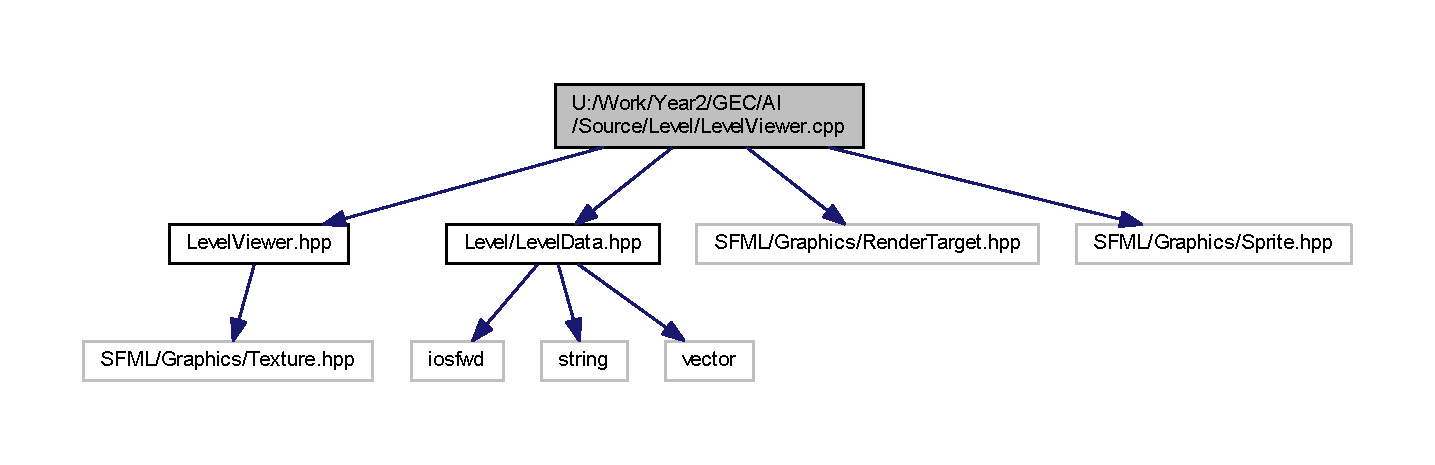
\includegraphics[width=350pt]{LevelViewer_8cpp__incl}
\end{center}
\end{figure}

\hypertarget{LevelViewer_8hpp}{\section{U\+:/\+Work/\+Year2/\+G\+E\+C/\+A\+I/\+Source/\+Level/\+Level\+Viewer.hpp File Reference}
\label{LevelViewer_8hpp}\index{U\+:/\+Work/\+Year2/\+G\+E\+C/\+A\+I/\+Source/\+Level/\+Level\+Viewer.\+hpp@{U\+:/\+Work/\+Year2/\+G\+E\+C/\+A\+I/\+Source/\+Level/\+Level\+Viewer.\+hpp}}
}
{\ttfamily \#include $<$S\+F\+M\+L/\+Graphics/\+Texture.\+hpp$>$}\\*
Include dependency graph for Level\+Viewer.\+hpp\+:
\nopagebreak
\begin{figure}[H]
\begin{center}
\leavevmode
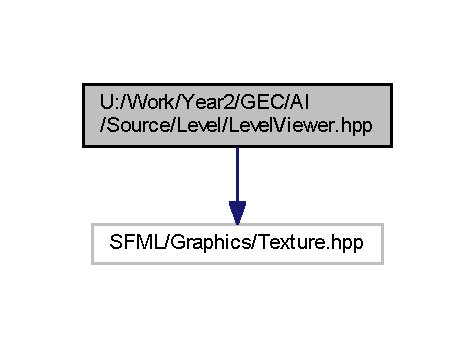
\includegraphics[width=228pt]{LevelViewer_8hpp__incl}
\end{center}
\end{figure}
This graph shows which files directly or indirectly include this file\+:
\nopagebreak
\begin{figure}[H]
\begin{center}
\leavevmode
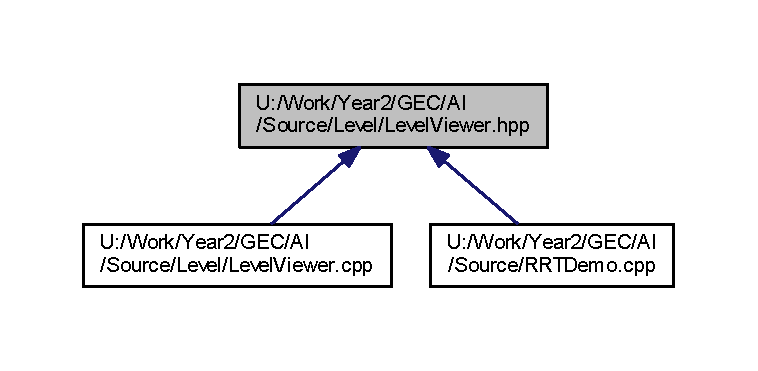
\includegraphics[width=350pt]{LevelViewer_8hpp__dep__incl}
\end{center}
\end{figure}
\subsection*{Classes}
\begin{DoxyCompactItemize}
\item 
class \hyperlink{classLevelViewer}{Level\+Viewer}
\begin{DoxyCompactList}\small\item\em A class used to display the contents of a \hyperlink{classLevelData}{Level\+Data} object on screen. \end{DoxyCompactList}\end{DoxyCompactItemize}

\hypertarget{RRT_8cpp}{\section{U\+:/\+Work/\+Year2/\+G\+E\+C/\+A\+I/\+Source/\+R\+R\+T/\+R\+R\+T.cpp File Reference}
\label{RRT_8cpp}\index{U\+:/\+Work/\+Year2/\+G\+E\+C/\+A\+I/\+Source/\+R\+R\+T/\+R\+R\+T.\+cpp@{U\+:/\+Work/\+Year2/\+G\+E\+C/\+A\+I/\+Source/\+R\+R\+T/\+R\+R\+T.\+cpp}}
}
{\ttfamily \#include \char`\"{}R\+R\+T.\+hpp\char`\"{}}\\*
{\ttfamily \#include $<$cassert$>$}\\*
{\ttfamily \#include $<$ctime$>$}\\*
{\ttfamily \#include $<$functional$>$}\\*
{\ttfamily \#include $<$random$>$}\\*
{\ttfamily \#include $<$utility$>$}\\*
{\ttfamily \#include $<$Level/\+Level\+Data.\+hpp$>$}\\*
Include dependency graph for R\+R\+T.\+cpp\+:
\nopagebreak
\begin{figure}[H]
\begin{center}
\leavevmode
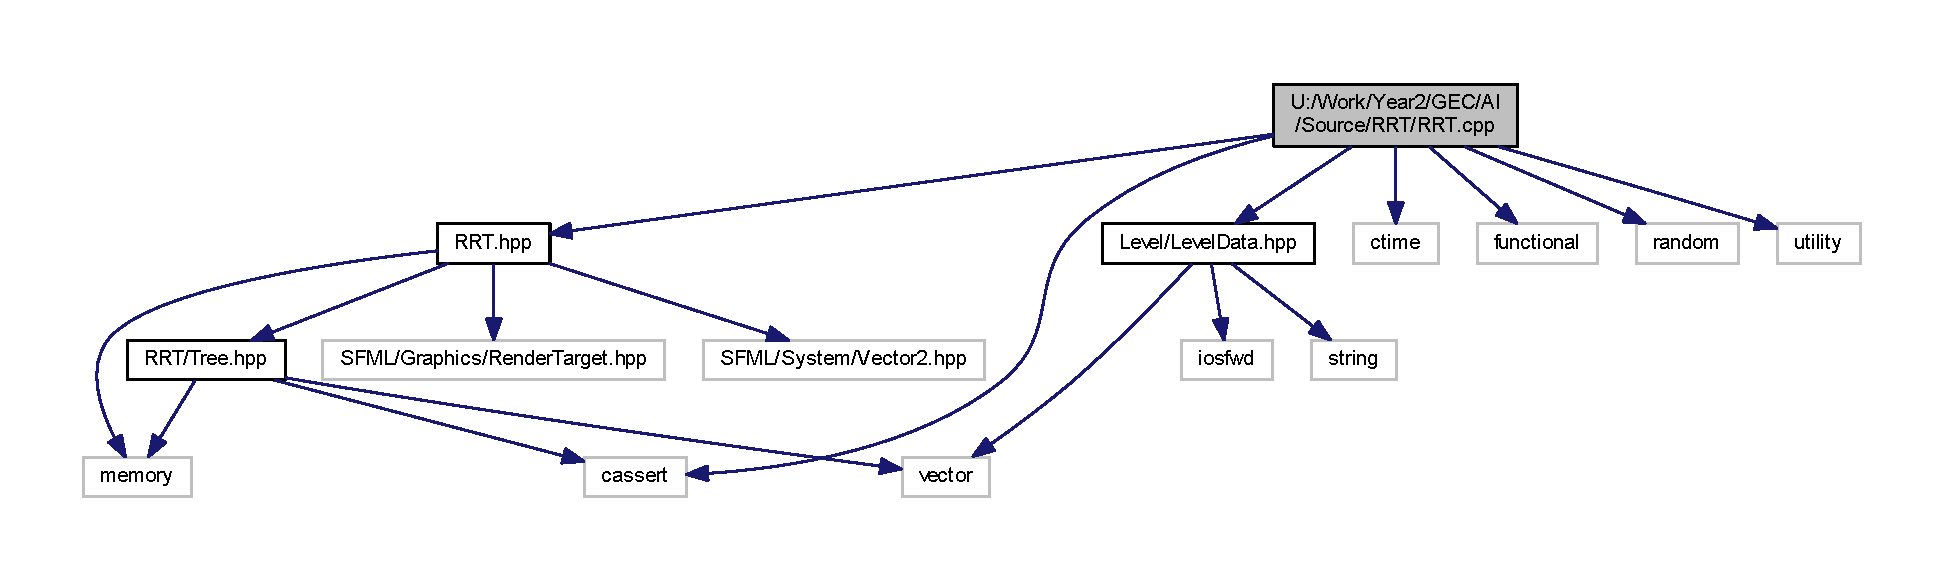
\includegraphics[width=350pt]{RRT_8cpp__incl}
\end{center}
\end{figure}

\hypertarget{RRT_8hpp}{\section{U\+:/\+Work/\+Year2/\+G\+E\+C/\+A\+I/\+Source/\+R\+R\+T/\+R\+R\+T.hpp File Reference}
\label{RRT_8hpp}\index{U\+:/\+Work/\+Year2/\+G\+E\+C/\+A\+I/\+Source/\+R\+R\+T/\+R\+R\+T.\+hpp@{U\+:/\+Work/\+Year2/\+G\+E\+C/\+A\+I/\+Source/\+R\+R\+T/\+R\+R\+T.\+hpp}}
}
{\ttfamily \#include $<$memory$>$}\\*
{\ttfamily \#include $<$R\+R\+T/\+Tree.\+hpp$>$}\\*
{\ttfamily \#include $<$S\+F\+M\+L/\+Graphics/\+Render\+Target.\+hpp$>$}\\*
{\ttfamily \#include $<$S\+F\+M\+L/\+System/\+Vector2.\+hpp$>$}\\*
Include dependency graph for R\+R\+T.\+hpp\+:
\nopagebreak
\begin{figure}[H]
\begin{center}
\leavevmode
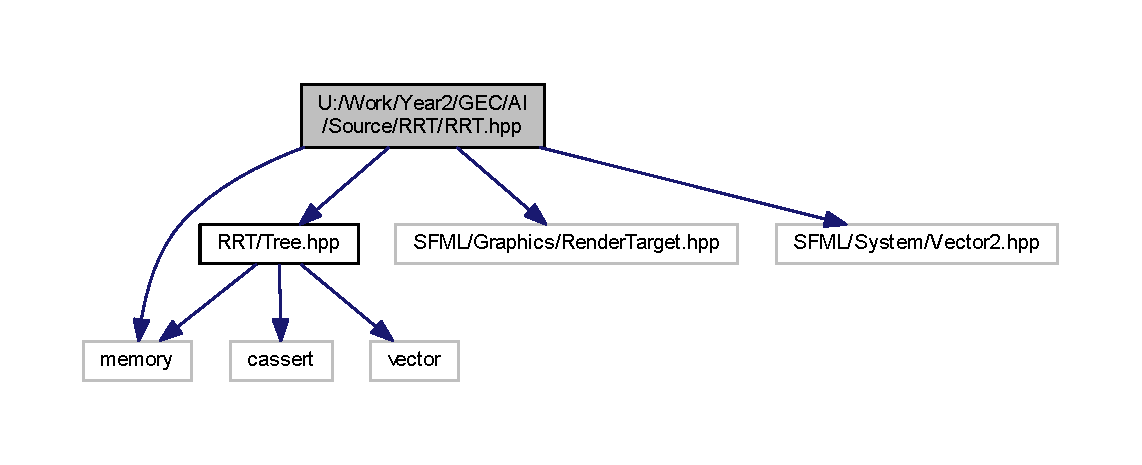
\includegraphics[width=350pt]{RRT_8hpp__incl}
\end{center}
\end{figure}
This graph shows which files directly or indirectly include this file\+:
\nopagebreak
\begin{figure}[H]
\begin{center}
\leavevmode
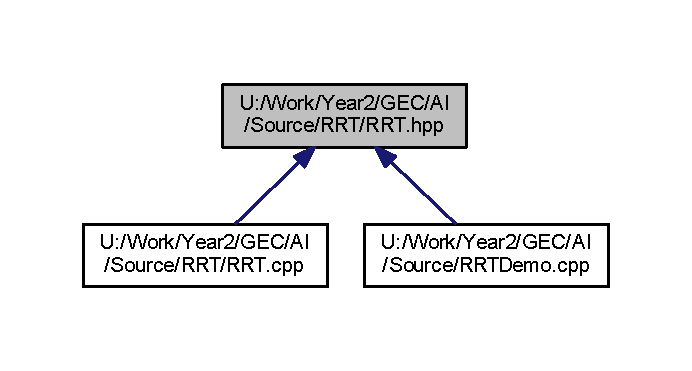
\includegraphics[width=332pt]{RRT_8hpp__dep__incl}
\end{center}
\end{figure}
\subsection*{Classes}
\begin{DoxyCompactItemize}
\item 
class \hyperlink{classRRT}{R\+R\+T}
\begin{DoxyCompactList}\small\item\em A class which creates an \hyperlink{classRRT}{R\+R\+T} tree when given a map and a start and end point. \end{DoxyCompactList}\end{DoxyCompactItemize}
\subsection*{Typedefs}
\begin{DoxyCompactItemize}
\item 
using \hyperlink{RRT_8hpp_ad96bf2a5632cc2b01900b403e90b1607}{R\+R\+T\+Tree} = char \hyperlink{classTree}{Tree}$<$ sf\+::\+Vector2i $>$
\end{DoxyCompactItemize}


\subsection{Typedef Documentation}
\hypertarget{RRT_8hpp_ad96bf2a5632cc2b01900b403e90b1607}{\index{R\+R\+T.\+hpp@{R\+R\+T.\+hpp}!R\+R\+T\+Tree@{R\+R\+T\+Tree}}
\index{R\+R\+T\+Tree@{R\+R\+T\+Tree}!R\+R\+T.\+hpp@{R\+R\+T.\+hpp}}
\subsubsection[{R\+R\+T\+Tree}]{\setlength{\rightskip}{0pt plus 5cm}using {\bf R\+R\+T\+Tree} =  char {\bf Tree}$<$sf\+::\+Vector2i$>$\hspace{0.3cm}{\ttfamily [strong]}}}\label{RRT_8hpp_ad96bf2a5632cc2b01900b403e90b1607}


Definition at line 21 of file R\+R\+T.\+hpp.


\hypertarget{Tree_8hpp}{\section{U\+:/\+Work/\+Year2/\+G\+E\+C/\+A\+I/\+Source/\+R\+R\+T/\+Tree.hpp File Reference}
\label{Tree_8hpp}\index{U\+:/\+Work/\+Year2/\+G\+E\+C/\+A\+I/\+Source/\+R\+R\+T/\+Tree.\+hpp@{U\+:/\+Work/\+Year2/\+G\+E\+C/\+A\+I/\+Source/\+R\+R\+T/\+Tree.\+hpp}}
}
{\ttfamily \#include $<$cassert$>$}\\*
{\ttfamily \#include $<$memory$>$}\\*
{\ttfamily \#include $<$vector$>$}\\*
Include dependency graph for Tree.\+hpp\+:
\nopagebreak
\begin{figure}[H]
\begin{center}
\leavevmode
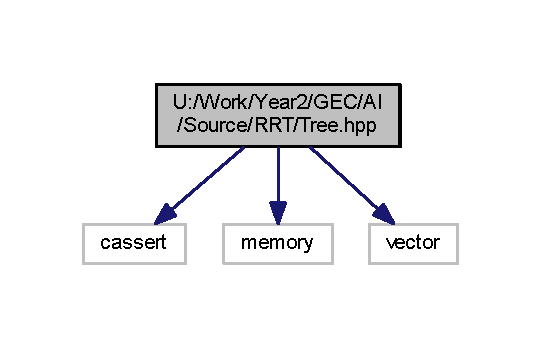
\includegraphics[width=260pt]{Tree_8hpp__incl}
\end{center}
\end{figure}
This graph shows which files directly or indirectly include this file\+:
\nopagebreak
\begin{figure}[H]
\begin{center}
\leavevmode
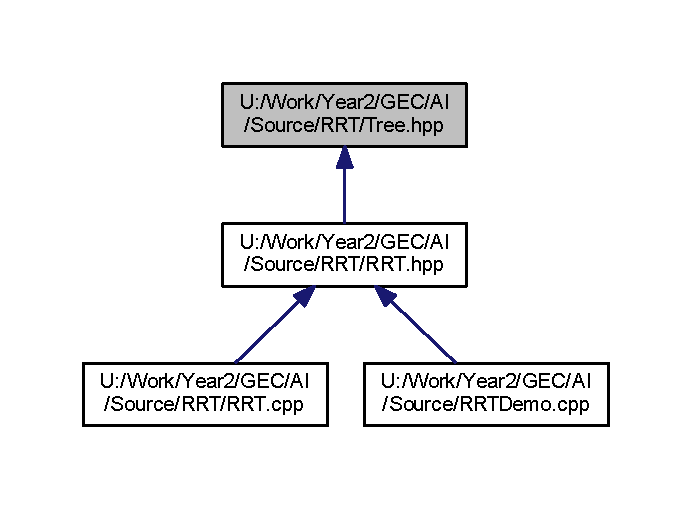
\includegraphics[width=332pt]{Tree_8hpp__dep__incl}
\end{center}
\end{figure}
\subsection*{Classes}
\begin{DoxyCompactItemize}
\item 
class \hyperlink{classTree}{Tree$<$ T $>$}
\begin{DoxyCompactList}\small\item\em A tree data structure containing a parent and an unlimited number of children. \end{DoxyCompactList}\end{DoxyCompactItemize}

\hypertarget{RRTDemo_8cpp}{\section{U\+:/\+Work/\+Year2/\+G\+E\+C/\+A\+I/\+Source/\+R\+R\+T\+Demo.cpp File Reference}
\label{RRTDemo_8cpp}\index{U\+:/\+Work/\+Year2/\+G\+E\+C/\+A\+I/\+Source/\+R\+R\+T\+Demo.\+cpp@{U\+:/\+Work/\+Year2/\+G\+E\+C/\+A\+I/\+Source/\+R\+R\+T\+Demo.\+cpp}}
}
{\ttfamily \#include \char`\"{}R\+R\+T\+Demo.\+hpp\char`\"{}}\\*
{\ttfamily \#include $<$utility$>$}\\*
{\ttfamily \#include $<$Level/\+Level\+Data.\+hpp$>$}\\*
{\ttfamily \#include $<$Level/\+Level\+Viewer.\+hpp$>$}\\*
{\ttfamily \#include $<$R\+R\+T/\+R\+R\+T.\+hpp$>$}\\*
{\ttfamily \#include $<$S\+F\+M\+L/\+Graphics/\+Render\+Window.\+hpp$>$}\\*
{\ttfamily \#include $<$S\+F\+M\+L/\+Window/\+Event.\+hpp$>$}\\*
Include dependency graph for R\+R\+T\+Demo.\+cpp\+:
\nopagebreak
\begin{figure}[H]
\begin{center}
\leavevmode
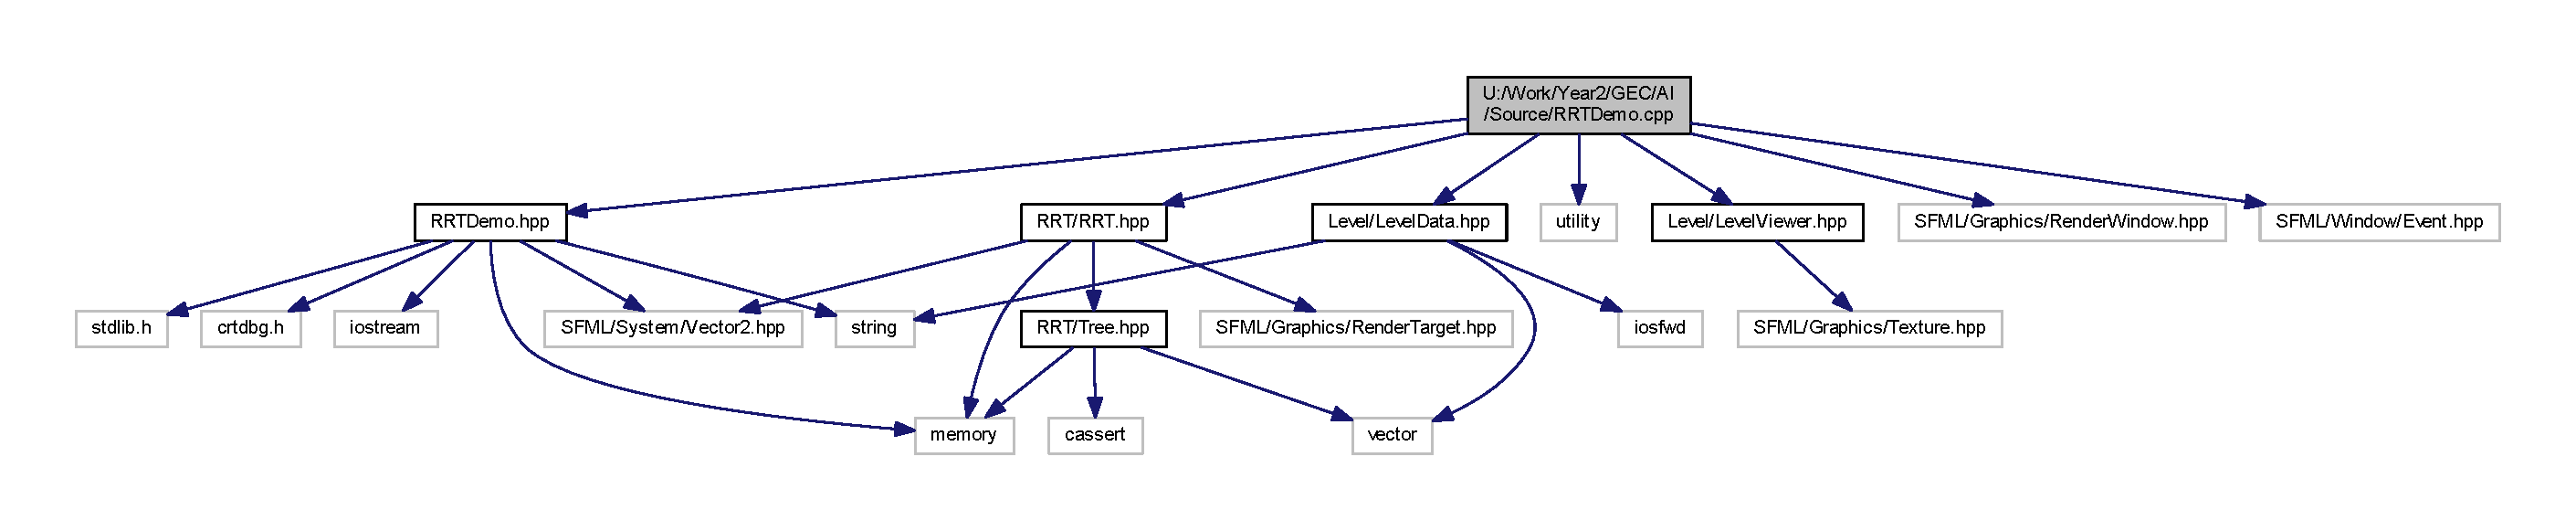
\includegraphics[width=350pt]{RRTDemo_8cpp__incl}
\end{center}
\end{figure}

\hypertarget{RRTDemo_8hpp}{\section{U\+:/\+Work/\+Year2/\+G\+E\+C/\+A\+I/\+Source/\+R\+R\+T\+Demo.hpp File Reference}
\label{RRTDemo_8hpp}\index{U\+:/\+Work/\+Year2/\+G\+E\+C/\+A\+I/\+Source/\+R\+R\+T\+Demo.\+hpp@{U\+:/\+Work/\+Year2/\+G\+E\+C/\+A\+I/\+Source/\+R\+R\+T\+Demo.\+hpp}}
}
{\ttfamily \#include $<$stdlib.\+h$>$}\\*
{\ttfamily \#include $<$crtdbg.\+h$>$}\\*
{\ttfamily \#include $<$iostream$>$}\\*
{\ttfamily \#include $<$memory$>$}\\*
{\ttfamily \#include $<$string$>$}\\*
{\ttfamily \#include $<$S\+F\+M\+L/\+System/\+Vector2.\+hpp$>$}\\*
Include dependency graph for R\+R\+T\+Demo.\+hpp\+:
\nopagebreak
\begin{figure}[H]
\begin{center}
\leavevmode
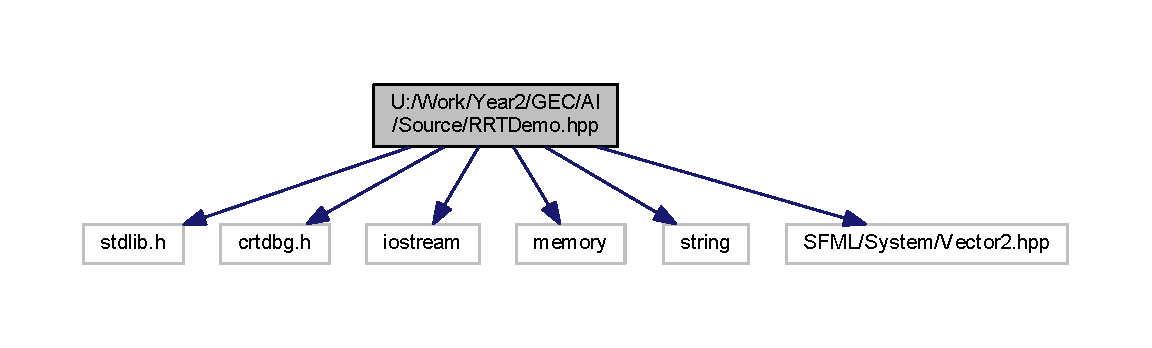
\includegraphics[width=350pt]{RRTDemo_8hpp__incl}
\end{center}
\end{figure}
This graph shows which files directly or indirectly include this file\+:
\nopagebreak
\begin{figure}[H]
\begin{center}
\leavevmode
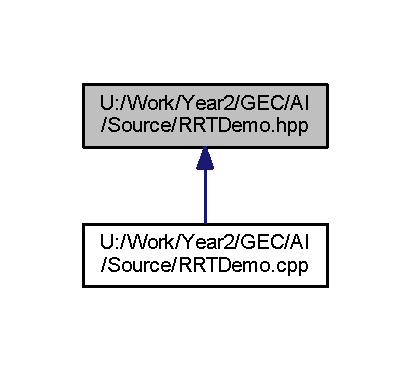
\includegraphics[width=197pt]{RRTDemo_8hpp__dep__incl}
\end{center}
\end{figure}
\subsection*{Classes}
\begin{DoxyCompactItemize}
\item 
class \hyperlink{classRRTDemo}{R\+R\+T\+Demo}
\begin{DoxyCompactList}\small\item\em A demo application which loads in level data from a file and uses the \hyperlink{classRRT}{R\+R\+T} algorithm to implement path finding. \end{DoxyCompactList}\end{DoxyCompactItemize}
\subsection*{Namespaces}
\begin{DoxyCompactItemize}
\item 
 \hyperlink{namespacesf}{sf}
\end{DoxyCompactItemize}
\subsection*{Macros}
\begin{DoxyCompactItemize}
\item 
\#define \hyperlink{RRTDemo_8hpp_afc30e481f763a8d68a861dba91be7316}{\+\_\+\+C\+R\+T\+D\+B\+G\+\_\+\+M\+A\+P\+\_\+\+A\+L\+L\+O\+C}
\end{DoxyCompactItemize}
\subsection*{Functions}
\begin{DoxyCompactItemize}
\item 
int \hyperlink{RRTDemo_8hpp_ae66f6b31b5ad750f1fe042a706a4e3d4}{main} ()
\begin{DoxyCompactList}\small\item\em The main function which starts the application. \end{DoxyCompactList}\end{DoxyCompactItemize}


\subsection{Macro Definition Documentation}
\hypertarget{RRTDemo_8hpp_afc30e481f763a8d68a861dba91be7316}{\index{R\+R\+T\+Demo.\+hpp@{R\+R\+T\+Demo.\+hpp}!\+\_\+\+C\+R\+T\+D\+B\+G\+\_\+\+M\+A\+P\+\_\+\+A\+L\+L\+O\+C@{\+\_\+\+C\+R\+T\+D\+B\+G\+\_\+\+M\+A\+P\+\_\+\+A\+L\+L\+O\+C}}
\index{\+\_\+\+C\+R\+T\+D\+B\+G\+\_\+\+M\+A\+P\+\_\+\+A\+L\+L\+O\+C@{\+\_\+\+C\+R\+T\+D\+B\+G\+\_\+\+M\+A\+P\+\_\+\+A\+L\+L\+O\+C}!R\+R\+T\+Demo.\+hpp@{R\+R\+T\+Demo.\+hpp}}
\subsubsection[{\+\_\+\+C\+R\+T\+D\+B\+G\+\_\+\+M\+A\+P\+\_\+\+A\+L\+L\+O\+C}]{\setlength{\rightskip}{0pt plus 5cm}\#define \+\_\+\+C\+R\+T\+D\+B\+G\+\_\+\+M\+A\+P\+\_\+\+A\+L\+L\+O\+C}}\label{RRTDemo_8hpp_afc30e481f763a8d68a861dba91be7316}


Definition at line 6 of file R\+R\+T\+Demo.\+hpp.



\subsection{Function Documentation}
\hypertarget{RRTDemo_8hpp_ae66f6b31b5ad750f1fe042a706a4e3d4}{\index{R\+R\+T\+Demo.\+hpp@{R\+R\+T\+Demo.\+hpp}!main@{main}}
\index{main@{main}!R\+R\+T\+Demo.\+hpp@{R\+R\+T\+Demo.\+hpp}}
\subsubsection[{main}]{\setlength{\rightskip}{0pt plus 5cm}int main (
\begin{DoxyParamCaption}
{}
\end{DoxyParamCaption}
)}}\label{RRTDemo_8hpp_ae66f6b31b5ad750f1fe042a706a4e3d4}


The main function which starts the application. 

\begin{DoxyReturn}{Returns}
The exit code of the application. 
\end{DoxyReturn}


Definition at line 104 of file R\+R\+T\+Demo.\+hpp.


%--- End generated contents ---

% Index
\newpage
\phantomsection
\addcontentsline{toc}{chapter}{Index}
\printindex

\end{document}
